% ==========================================================================================================================
%________/\\\\\\\\\__/\\\\\\\\\\\\\____/\\\\____________/\\\\_        
% _____/\\\////////__\/\\\/////////\\\_\/\\\\\\________/\\\\\\_       
%  ___/\\\/___________\/\\\_______\/\\\_\/\\\//\\\____/\\\//\\\_      
%   __/\\\_____________\/\\\\\\\\\\\\\\__\/\\\\///\\\/\\\/_\/\\\_     
%    _\/\\\_____________\/\\\/////////\\\_\/\\\__\///\\\/___\/\\\_    
%     _\//\\\____________\/\\\_______\/\\\_\/\\\____\///_____\/\\\_   
%      __\///\\\__________\/\\\_______\/\\\_\/\\\_____________\/\\\_  
%       ____\////\\\\\\\\\_\/\\\\\\\\\\\\\/__\/\\\_____________\/\\\_ 
%        _______\/////////__\/////////////____\///______________\///__
% ==========================================================================================================================

\section{Экспериментальная установка CBM}\label{sec:secCbmSetup}

\bigskip

Эксперимент CBM нацелен на исследование сжатой барионной материи с высокой плотностью и относительно низкой температурой с помощью редких наблюдаемых. К этим наблюдаемым относятся легкие векторные мезоны, частицы со скрытым и открытым очарованием, прецизионно измеренные анизотропии в угловых и энергетических распределениях, а в случае реализации фазового перехода первого рода --- флуктуации различных параметров от события к событию. Для реализации такой физической программы необходимо добиться рекордно высокой частоты взаимодействий. Эксперимент строится по схеме с фиксированной мишенью с интенсивностью пучка до $10^9$~с$^{-1}$ и энергией, например, для золота --- до 11~\GeVperNucl{} на SIS100. За счёт использования тонкой мишени, обеспечивающей ядерные взаимодействия с вероятностью $\approx$1\% частота последних будет достигать $10^7$~с$^{-1}$. Благодаря работе с фиксированной мишенью, большинство вторичных частиц будут лететь вперед. Отметим, что ионы, проходящие через мишень без ядерного взаимодействия, рождают большое количество дельта-электронов, дающих значительные фоны в некоторых подсистемах. Детектор оказывается в довольно жестких условиях эксплуатации. С одной стороны, имеют место высокие градиенты угловой плотности частиц, с другой стороны, наблюдаются высокие частоты взаимодействий. Таким образом, детектор должен быть спроектирован с учетом требований переменной гранулярности, высокой радиационной стойкости и способности обрабатывать большой поток данных. Последнее требование достигается путем использования самозапускающейся электроники. В таком подходе каждый канал электроники вырабатывает сообщение при условии преодоления сигналом некоторого порога. Сообщение содержит в общем случае идентификатор сработавшего канала, временную отметку и амплитудную информацию. После срабатывания каналы на некоторое время теряют чувствительность, а остальные каналы продолжают ожидать следующее событие. В результате при регистрации каждого события имеется некоторое количество случайно распределенных нечувствительных каналов, что приводит к необходимости устойчивости алгоритмов реконструкции к пропущенным хитам. Это касается как треков частиц в различных комбинациях детекторов, так и черенковских колец. Ниже обсуждаются особенности компоновки и конструктивных решений различных подсистем эксперимента.

%Установка CBM --- основной инструмент для проведения исследований плотной барионной материи на FAIR.
Для выполнения различных измерений CBM будет функционировать в двух конфигурациях --- с мюонным детектором (MUCH) и с детектором черенковских колец (RICH). Схема экспериментальной установки с RICH представлена на \figref{fig:CBM}.

\begin{figure}[H]
\centering
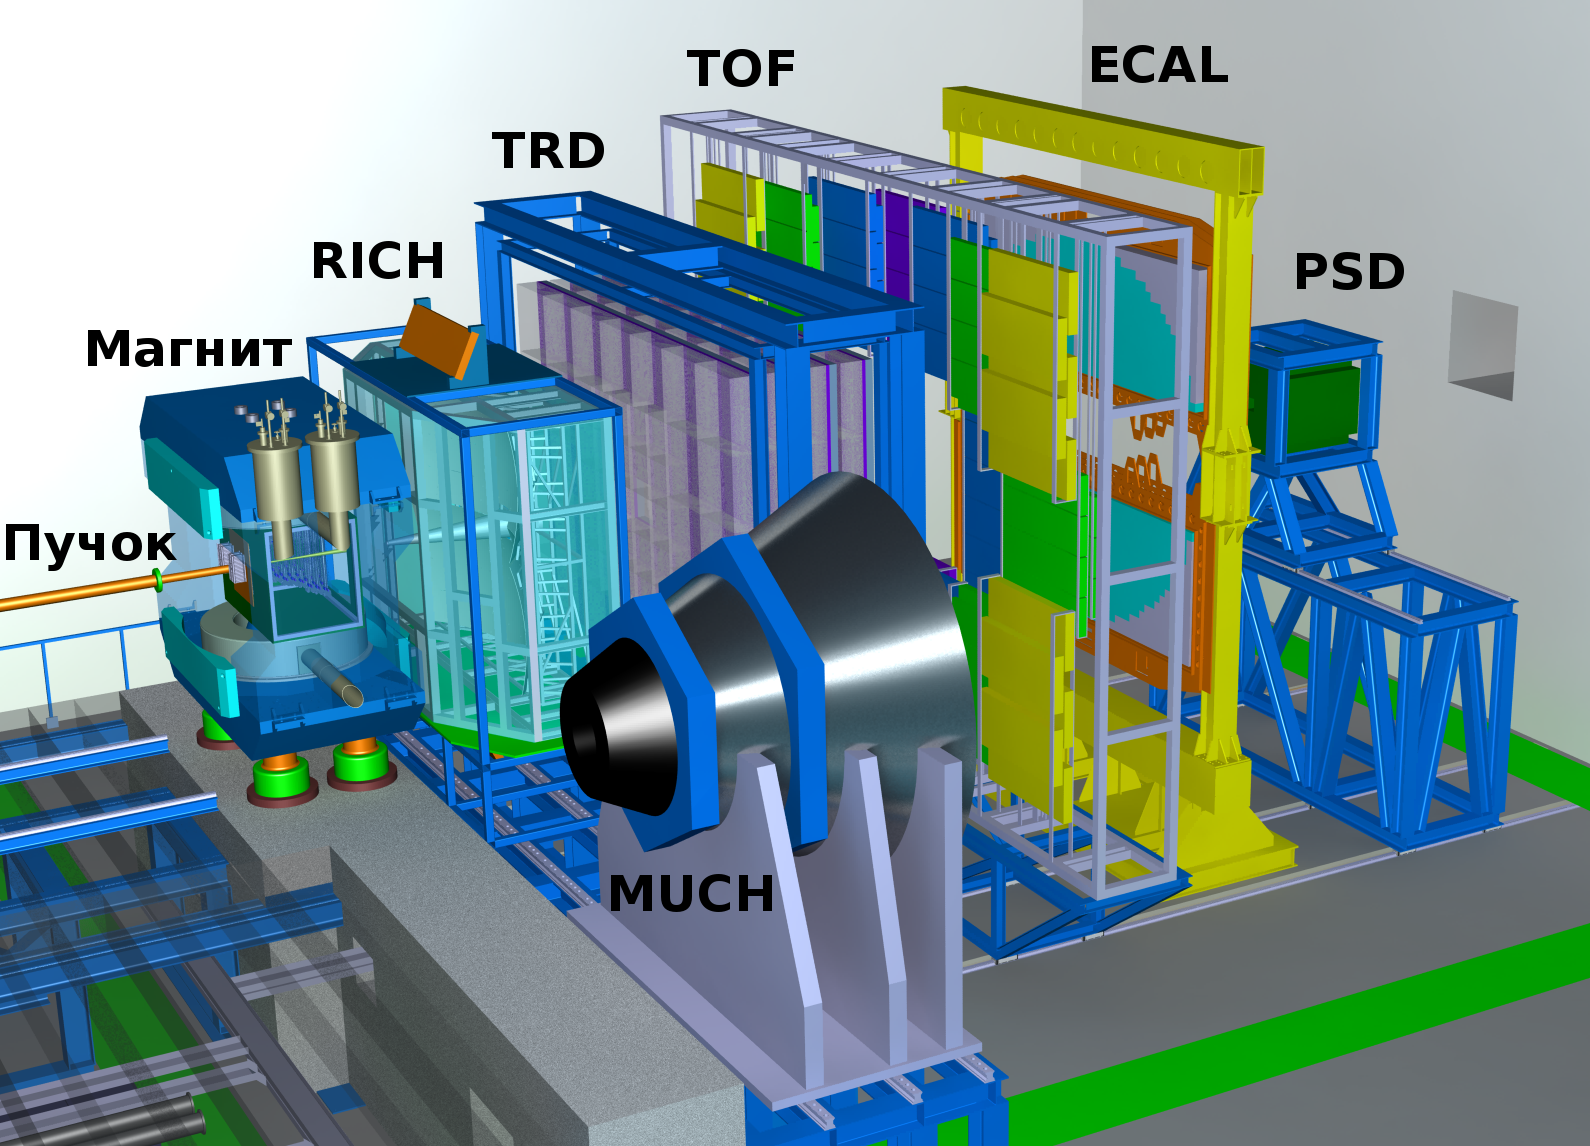
\includegraphics[width=1.0\textwidth]{pictures/1_CBM_SIS100_with_names.png}
\caption{Общий вид экспериментальной установки CBM в конфигурации с RICH. MUCH показан в нерабочем положении.}
\label{fig:CBM}
\end{figure}

%(см.~\figref{fig:InMagnetBox}) 

Между полюсами сверхпроводящего дипольного магнита~\cite{TDR_Magnet} расположена вакуумная камера, содержащая мишень и вершинный микродетектор (MVD)~\cite{MVD_KOZIEL}, выполненный на основе монолитного пиксельного детектора типа MAPS. Ниже по пучку также между полюсами, но уже вне вакуумной камеры, располагаются станции кремниевой трековой системы (STS)~\cite{TDR_STS}, собранные из двухсторонних микростриповых сенсоров. Координатные трековые детекторы MVD и STS предназначены для реконструкции траекторий заряженных частиц, восстановления их импульсов и нахождения вторичных вершин в условиях высокой множественности и плотности частиц.

% с точностью не хуже 1\% (выпилено)

%\begin{figure}[H]
%\centering
%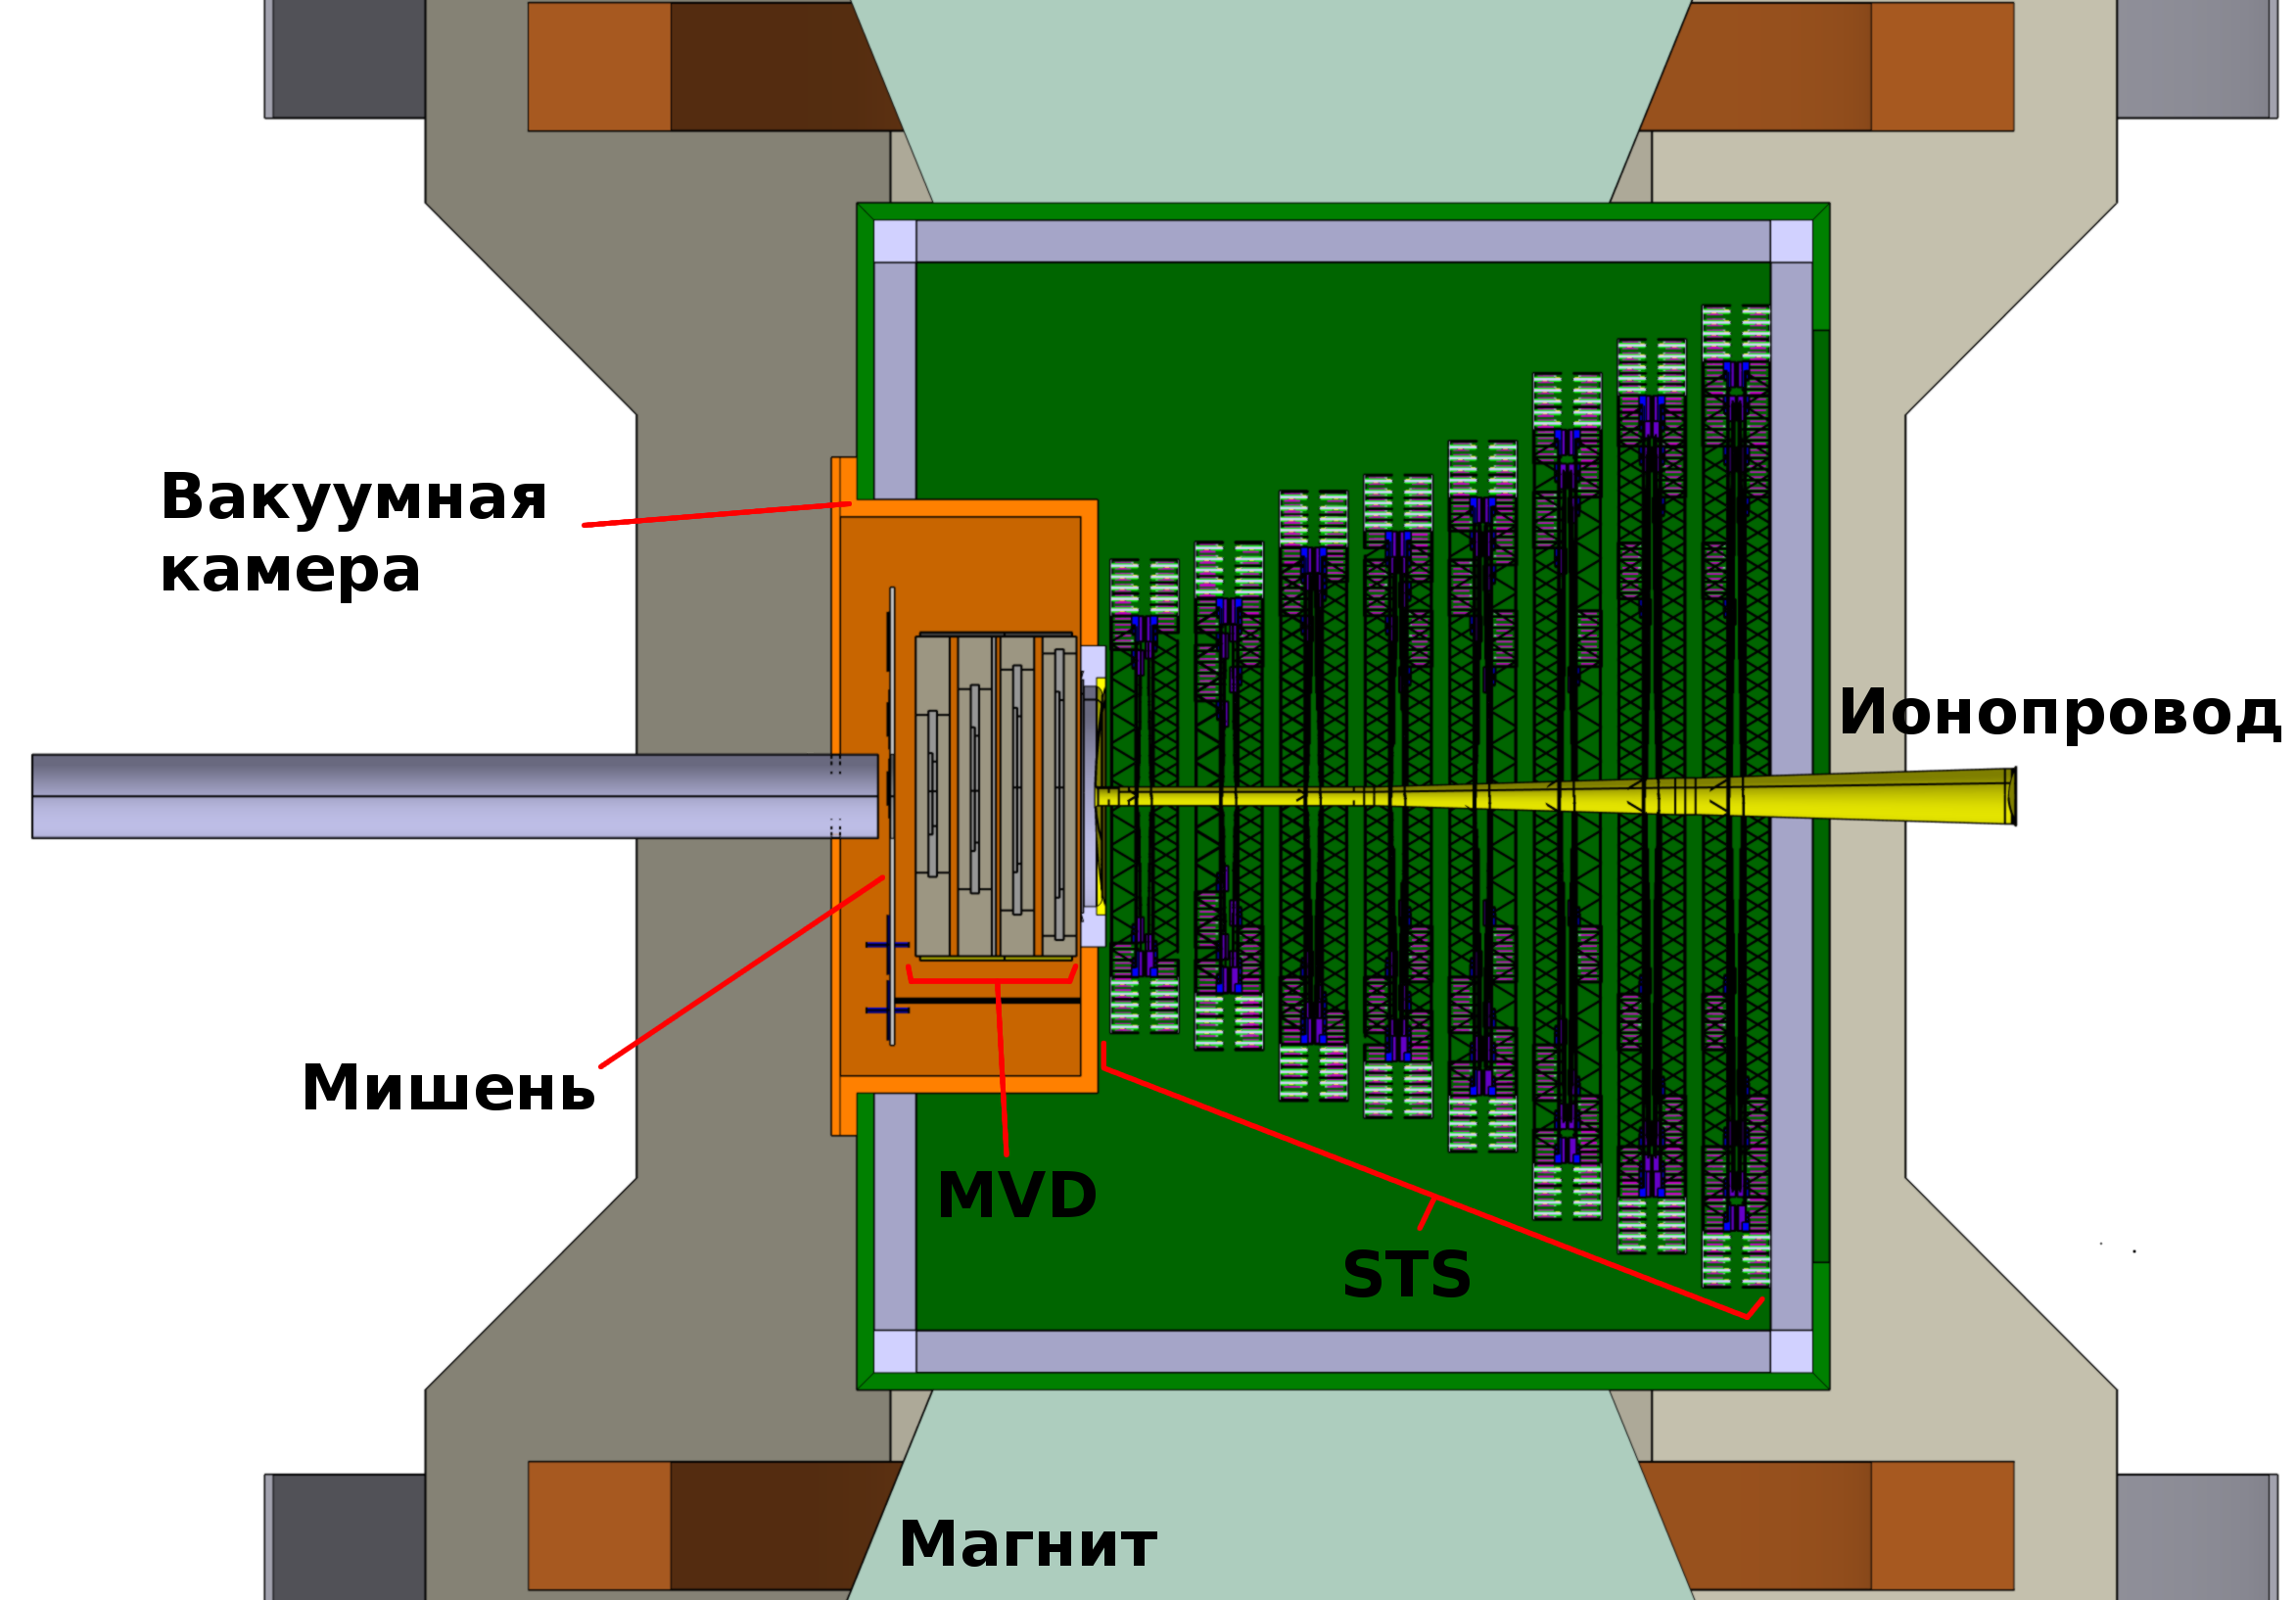
\includegraphics[width=0.8\textwidth]{pictures/CBM_vacuum_chamber_model.png}
%\caption{Разрез модели ионопровода, вакуумной камеры и детекторов, расположенных между полюсами магнита.}
%\label{fig:InMagnetBox}
%\end{figure}

Следом за STS в рассматриваемой конфигурации расположен детектор черенковских колец (RICH)~\cite{TDR_RICH}, предназначенный для идентификации электронов и позитронов в диапазоне импульсов от 0.5~\GeVoverC{} до 8~\GeVoverC{} с целью восстановления распадов лёгких векторных мезонов и частиц со скрытым очарованием. Во второй конфигурации на месте RICH стоит мюонная система (MUCH, показана на \figref{fig:CBM} в нерабочем положении)~\cite{TDR_MUCH}, предназначенная в первую очередь для исследования частиц, распадающихся по димюонному каналу, и состоящая из чередующихся слоев железа и газовых трековых камер~\cite{GEM}.

Детектор переходного излучения (TRD) используется для реконструкции треков частиц и идентификации электронов/позитронов в условиях доминирующего фона от $\pi$-мезонов~\cite{TRD}. Для идентификации адронов используется время-пролётный детектор (TOF)~\cite{TDR_TOF}. Электромагнитный калориметр (ECAL) типа ``шашлык'' необходим для регистрации прямых фотонов и фотонов от распада нейтральных мезонов ($ \pi^{0}, \eta $)~\cite{ECAL_KOROLKO}. Детектор непровзаимодействовавших осколков ядер (PSD)~\cite{TDR_PSD} представляет собой сегментированный адронный калориметр и служит для определения центральности столкновения и плоскости реакции путем регистрации ядерных осколков, летящих под малыми углами к пучку.

Детекторы CBM будут оборудованы самотриггирующейся электроникой, а построение и отбор событий будет осуществляться с помощью специализированного аппаратно-программного комплекса FLES.

Различные комбинации детекторов будут использоваться при измерении различных наблюдаемых, см. таблицу~\ref{tabl:CBMdetectorsAndObservables}.

% \begin{tabular}{ | p{0.2\linewidth} | p{0.07\linewidth} | p{0.07\linewidth} | p{0.07\linewidth} | p{0.07\linewidth} | p{0.07\linewidth} | p{0.07\linewidth} | p{0.07\linewidth} | p{0.07\linewidth} | }

\begin{table}[H]
\caption{Наблюдаемые и детекторы для их регистрации. Детекторы, помеченные x, необходимы для регистрации соответствующих частиц, а детекторы, помеченные (x), могут использоваться для подавления фона.}
\label{tabl:CBMdetectorsAndObservables}
\begin{tabular}{ | p{0.2\linewidth} | c | c | c | c | c | c | c | c | c | }
\hline
\textbf{Тип частиц} & \textbf{MVD} & \textbf{STS} & \textbf{RICH} & \textbf{MUCH} & \textbf{TRD} & \textbf{TOF} & \textbf{ECAL} & \textbf{PSD} \\
\hline
$\pi$, $K$, $p$ & & x & (x) &  & (x) & x &  & x \\
\hline
Гипероны & & x & & & (x) & (x) & & x \\ 
\hline
Частицы с открытым очарованием & x & x & (x) & & (x) & x & & x\\
\hline
Электроны & x & x & x & & x & x & & x \\
\hline
Мюоны & & x & & x & & (x) & & x \\
\hline
Гамма & & & & & & & x & x \\
\hline
Гамма через $e^{\pm}$ конверсию & x & x & x & & x & x & & x \\
\hline
\end{tabular}
\end{table}

Далее каждая подсистема установки описана подробнее.

% ==========================================================================================================================
%_______/\\\\\_______/\\\\\\\\\\\\\\\__/\\\________/\\\__/\\\\\\\\\\\\\\\____/\\\\\\\\\_____        
% _____/\\\///\\\____\///////\\\/////__\/\\\_______\/\\\_\/\\\///////////___/\\\///////\\\___       
%  ___/\\\/__\///\\\________\/\\\_______\/\\\_______\/\\\_\/\\\_____________\/\\\_____\/\\\___      
%   __/\\\______\//\\\_______\/\\\_______\/\\\\\\\\\\\\\\\_\/\\\\\\\\\\\_____\/\\\\\\\\\\\/____     
%    _\/\\\_______\/\\\_______\/\\\_______\/\\\/////////\\\_\/\\\///////______\/\\\//////\\\____    
%     _\//\\\______/\\\________\/\\\_______\/\\\_______\/\\\_\/\\\_____________\/\\\____\//\\\___   
%      __\///\\\__/\\\__________\/\\\_______\/\\\_______\/\\\_\/\\\_____________\/\\\_____\//\\\__  
%       ____\///\\\\\/___________\/\\\_______\/\\\_______\/\\\_\/\\\\\\\\\\\\\\\_\/\\\______\//\\\_ 
%        ______\/////_____________\///________\///________\///__\///////////////__\///________\///__
% ==========================================================================================================================

\subsection{Вакуумная камера, мишень и ионопровод}\label{sec:secVacChamberPipe}

%CBM является экспериментом с фиксированной мишенью.
Пучок подводится к установке с помощью ионопровода, который стыкуется с вакуумной камерой, расположенной между полюсами дипольного магнита. Внутри вакуумной камеры находится мишень и вершинный микродетектор MVD. Мишень представляет собой фольгу из золота или другого материала толщиной порядка ста микрон или набор из нескольких фольг меньшей толщины, разнесённых вдоль оси пучка. Непровзаимодействовавшие ионы налетающего пучка и крупные осколки продолжают движение по ионопроводу за вакуумной камерой.

Планируется, что пучковая труба будет выполнена из алюминия толщиной от 0.3~мм и диаметром от 4~см на выходе из вакуумной камеры до 60~см в зоне время-пролётного детектора.

Для измерения момента времени первичного взаимодействия пучка с мишенью, который необходим для измерения времени пролёта вторичных частиц с помощью TOF, вблизи мишени будет расположен стартовый детектор. См. также~\ref{sec:secTOF}.

% ==========================================================================================================================
%__/\\\\____________/\\\\__/\\\________/\\\__/\\\\\\\\\\\\____        
% _\/\\\\\\________/\\\\\\_\/\\\_______\/\\\_\/\\\////////\\\__       
%  _\/\\\//\\\____/\\\//\\\_\//\\\______/\\\__\/\\\______\//\\\_      
%   _\/\\\\///\\\/\\\/_\/\\\__\//\\\____/\\\___\/\\\_______\/\\\_     
%    _\/\\\__\///\\\/___\/\\\___\//\\\__/\\\____\/\\\_______\/\\\_    
%     _\/\\\____\///_____\/\\\____\//\\\/\\\_____\/\\\_______\/\\\_   
%      _\/\\\_____________\/\\\_____\//\\\\\______\/\\\_______/\\\__  
%       _\/\\\_____________\/\\\______\//\\\_______\/\\\\\\\\\\\\/___ 
%        _\///______________\///________\///________\////////////_____
% ==========================================================================================================================

\subsection{Вершинный микродетектор MVD}\label{sec:secMVD}

\begin{minipage}[t]{0.495\textwidth}

Вершинный микродетектор (Micro Vertex Detector, MVD) является первым трекинговым устройством установки CBM и расположен внутри вакуумной камеры (см.~\figref{fig:MVD1}). MVD состоит из четырёх двухсторонних станций, расположенных на расстояниях 5, 10, 15 и 20~см от мишени вниз по пучку.
MVD улучшает разрешение трековой системы CBM, позволяя таким образом идентифицировать редкие частицы по пространственному отклонению вершины распада от точки взаимодействия налетающего иона и ядра мишени. В таблице~\ref{tabl:MVDphys} приведены наблюдаемые, измерение которых возможно за счёт использования MVD.
Помимо этого, широкий геометрический аксептанс MVD вносит значительный вклад в трекинг частиц с низким импульсом, что повышает способность системы к подавлению фона при измерении распадов по дилептонному каналу.
\end{minipage}
\begin{minipage}[t]{0.495\textwidth}
\begin{figure}[H]
\centering
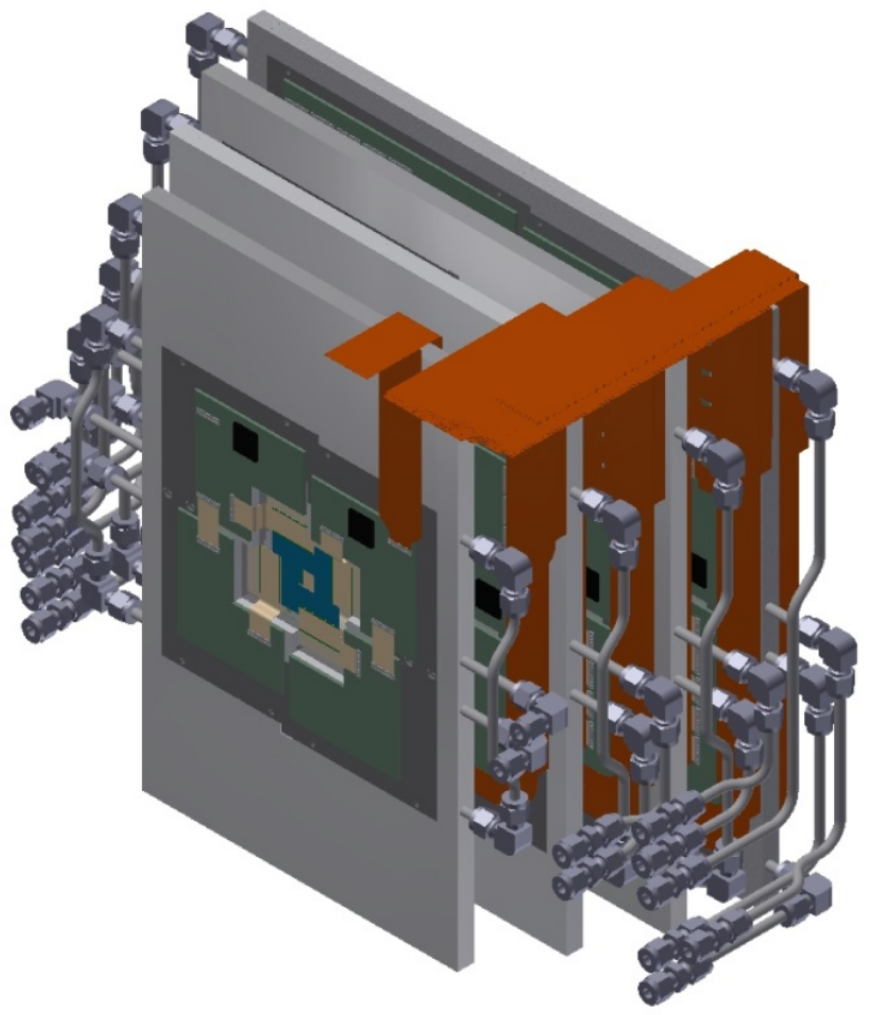
\includegraphics[width=0.9\textwidth]{pictures/MVD_1.png}
\caption{Модель вершинного микродетектора.}
\label{fig:MVD1}
\end{figure}
\end{minipage}

\begin{table}[H]
\caption{}
\label{tabl:MVDphys}
\begin{tabular}{ | p{0.22\linewidth} | p{0.22\linewidth} | p{0.22\linewidth} | p{0.22\linewidth} | }
\hline
\textbf{Частица} & \textbf{Канал} \newline \textbf{распада} & \textbf{Коэф.} \newline \textbf{ветвления} & \textbf{Время жизни, c$\tau$} \\
\hline
$\mathbf{D^{+}}$ & $K^{-} + \pi^{+} + \pi^{+}$ & 9\% & $315$~мкм \\
\hline
$\mathbf{D^{0}}$ & $K^{-} + \pi^{+}$ & 4\% & $124$~мкм \\
\hline
$\mathbf{\lambda_{C}}$ & $p + K^{-} + \pi^{+}$ & 5\% & $62$~мкм \\
\hline
\end{tabular}
\end{table}

MVD будет построен на основе активных пиксельных КМОП (CMOS) сенсоров (Monolithic Active Pixel Sensors, MAPS) толщиной $50$~мкм, имеющих пространственное разрешение $3.5$~мкм. Данная технология, вместе с правильно подобранными материалами для опорных структур и кабелей, позволяет получить толщину материала порядка 0.3\%~$X_{0}$ для первой станции.

%\small{The Micro Vertex Detector (MVD) is the first tracking device, with its first station located only 5 cm downstream of the fixed target. It will improve the vertex resolution of the CBM tracking system, to be able to identify rare particles by the spatial displacement of their decay vertices. In addition, the large geometrical acceptance of the MVD will significantly contribute to the tracking of low-momentum particles and thus improve the background suppression capability in dielectron measurements. The MVD employs highly granular, 50 $\mu$m thin CMOS Pixel Sensors. Together with high performance carrier materials and cable technology, this results in a material budget of only 0.3\% $X_{0}$ for the first station.}

%\small{The MVD will rely on CMOS Monolithic Active Pixel Sensors (MAPS) which provide the necessary radiation tolerance, a spatial resolution of 3.5$\mu$m, 50$\mu$m thickness, and advanced on-chip data processing.}

%\small{The MVD will operate in the target vacuum to obtain the best possible vertex resolution.}

На~\figref{fig:MVD23} показано устройство сенсора MVD.
На части чипа сенсора реализована предварительная обработка сигнала.
По тонким гибким шлейфам к сенсорам подводится питание и осуществляется считывание.
За пределами геометрического аксептанса расположены платы передней электроники и система жидкостного охлаждения, соединённая с сенсорами с помощью пластины из CVD алмаза.
Данные (800~Mbps/сенсор) считываются радиационно-стойкими пассивными платами передней электроники и отправляются в DAQ-систему по стандарту HADES-TRB3.
%Детектор MVD будет испытывать значительные радиационные нагрузки, поэтому о
Особое внимание уделяется охлаждению активных сенсоров.

При всех своих достоинствах MAPS --- это довольно-таки медленный детектор, поэтому для работы с ним частота взаимодействий должна быть снижена до $10^5$--$10^6$~Гц.

%\small{A part of the sensor chip hosts data processing circuits. The second sensor covers this surface.}
%\small{Thin flex print cables serve to bias and readout the sensors.}
%\small{A liquid cooled heat sink located outside the detector acceptance hosts front end boards and absorbs the dissipated power of the system}
%\small{The data of the sensors will be received by a radiation tolerant, passive front end board. It sends the data (800~Mbps/sensor) to a DAQ-system based on the HADES-TRB3 standard.}

%\textbf{Какие-то слова о системе считывания, пока что аналогичной той, что используется в RICH. Временное разрешение $5$~мкс \todo \todo \todo}

\begin{figure}[H]
\centering
%\begin{minipage}[b]{0.395\textwidth}
%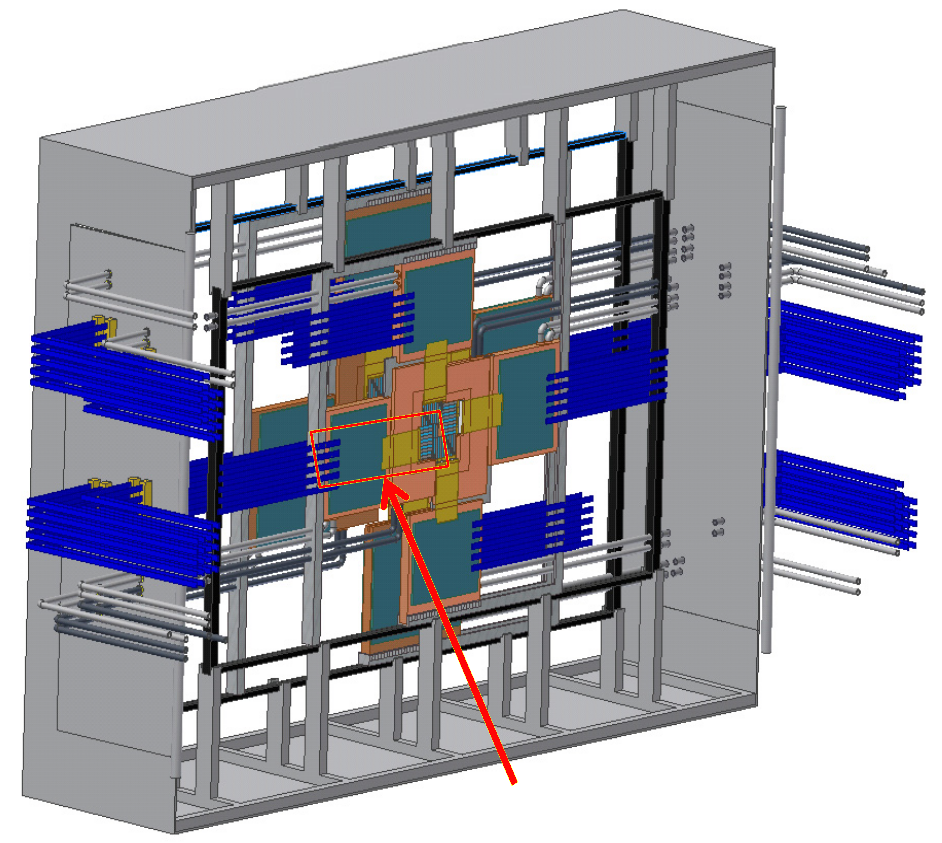
\includegraphics[width=0.95\textwidth]{pictures/MVD_2.png}
%\end{minipage}
%\hspace{0.01\textwidth}
%\begin{minipage}[b]{0.595\textwidth}
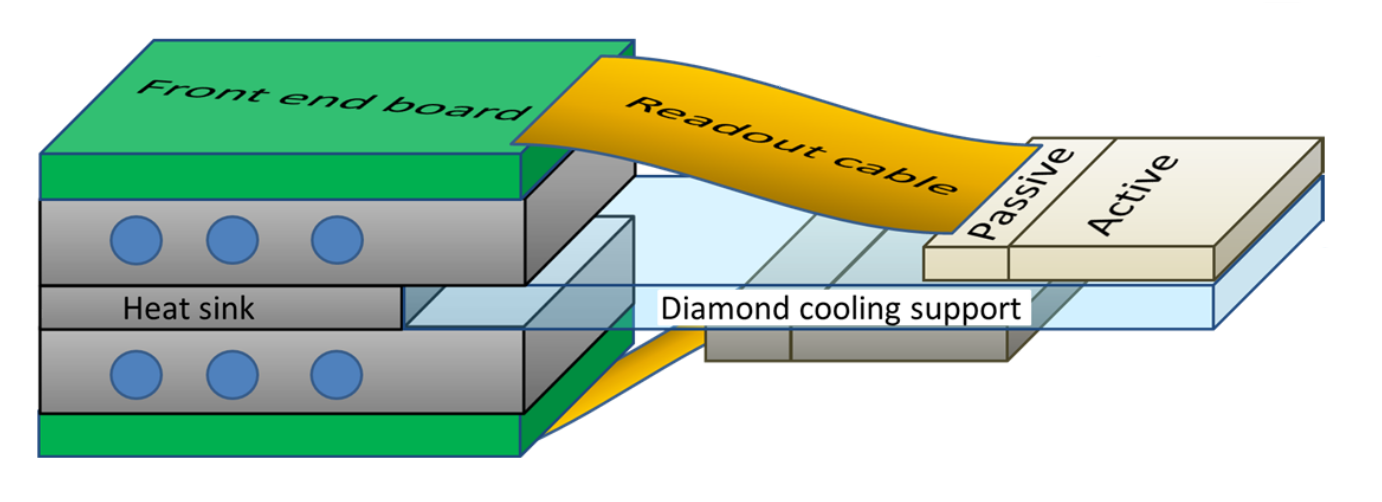
\includegraphics[width=0.7\textwidth]{pictures/MVD_3.png}
%\end{minipage}
\caption{Конструкция сенсора MVD }
\label{fig:MVD23}
\end{figure}

% ==========================================================================================================================
%_____/\\\\\\\\\\\____/\\\\\\\\\\\\\\\_____/\\\\\\\\\\\___        
% ___/\\\/////////\\\_\///////\\\/////____/\\\/////////\\\_       
%  __\//\\\______\///________\/\\\________\//\\\______\///__      
%   ___\////\\\_______________\/\\\_________\////\\\_________     
%    ______\////\\\____________\/\\\____________\////\\\______    
%     _________\////\\\_________\/\\\_______________\////\\\___   
%      __/\\\______\//\\\________\/\\\________/\\\______\//\\\__  
%       _\///\\\\\\\\\\\/_________\/\\\_______\///\\\\\\\\\\\/___ 
%        ___\///////////___________\///__________\///////////_____
% ==========================================================================================================================

\subsection{Кремниевая трековая система STS}\label{sec:secSTS}

% From CBM STS TDR Summary

Задача кремниевой трековой системы (Silicon Tracking System, STS), изображённой на~\figref{fig:STS12} --- измерение траекторий и импульсов заряженных частиц, вылетающих из точки взаимодействия пучка тяжёлых ионов с мишенью. Для выполнения физической программы CBM необходима частота взаимодействий до 10~МГц, при том что в одном взаимодействии будет рождаться до 1000 заряженных частиц. Реконструкция треков должна выполняться с эффективностью порядка 95\% и разрешением по импульсу порядка $\Delta p / p = 1\%$.

%\small{The detector system’s task is to measure the trajectories and momenta of charged particles originating from the interactions of heavy-ion beams with nuclear targets. Up to 1000 charged particles are produced per interaction, at rates up to 10 MHz to enable CBM physics with rare observables. The track reconstruction has to be achieved with 95\% efficiency and a momentum resolution $\Delta p / p = 1\%$. These requirements can be fulfilled with a tracking system of 8 low-mass layers of silicon microstrip sensors located at distances between 30 cm and 100 cm downstream of the target inside the magnetic dipole field.}

STS будет состоять из 8~слоёв кремниевых микростриповых сенсоров, расположенных внутри магнитного поля на расстоянии от 30~см до 100~см от точки взаимодействия вниз по пучку с шагом 10~см.
Микростриповые сенсоры будут двухсторонними, шаг между стрипами $58$~мкм, стерео-угол \SI{7.5}{\degree}, длина стрипов в различных сенсорах от 20~до~60~мм, а толщина кремния $300$~мкм.

По текущим оценкам максимальная неионизирующая доза в CBM для сенсоров, расположенных ближе всего к пучку, не будет превышать $10^{14}$ $n_{eq}$ см$^{-2}$.
Сенсоры будут монтироваться на лёгкие карбоновые фермы. Считывание будет осуществляться по многоканальным микро-кабелям самотриггирующейся электроникой, расположенной по краям станций вместе с линиями охлаждения и другими инфраструктурными подсистемами.
Многослойные полиамид-алюминиевые кабели будут иметь толщину порядка $100$~мкм.
STS будет работать в термостатическом корпусе (см.~\figref{fig:STS12}), обеспечивающем постоянную температуру около \SI{-5}{\degreeCelsius}. Тепло, рассеиваемое считывающей электроникой, отводится с помощью $CO_{2}$ системы охлаждения. Механические опоры детектора и соединения спроектированы так, чтобы была возможность заменить отдельный модуль системы не отсоединяя остальные.

%\small{The sensors are mounted onto lightweight mechanical support ladders and read out through multi-line micro-cables with fast self-triggering electronics at the periphery of the stations where cooling lines and other infrastructure can be placed. The micro-cables will be built from sandwiched polyimide-Aluminum layers of several 10~$\mu$m thickness. The microstrip sensors will be double-sided with a stereo angle of \SI{7.5}{\degree}, a strip pitch of 58~$\mu$m, strip lengths between 20 and 60 mm, and a thickness of 300 $\mu$m of silicon. According to the CBM running scenario the maximum non-ionizing dose for the sensors closest to the beam line does not exceed $10^{14}$ $n_{eq}$ см$^{-2}$. The STS is operated in a thermal enclosure that keeps the sensors at a temperature of about \SI{-5}{\degreeCelsius}. The heat dissipated in the read-out electronics is removed by a $CO_{2}$ cooling system. The mechanical structure of the detector system including the service and signal connections is designed such that single detector ladders can be exchanged without disconnecting and removing more than one detector station.}

\begin{figure}[H]
\centering
%\begin{minipage}[b]{0.495\textwidth}
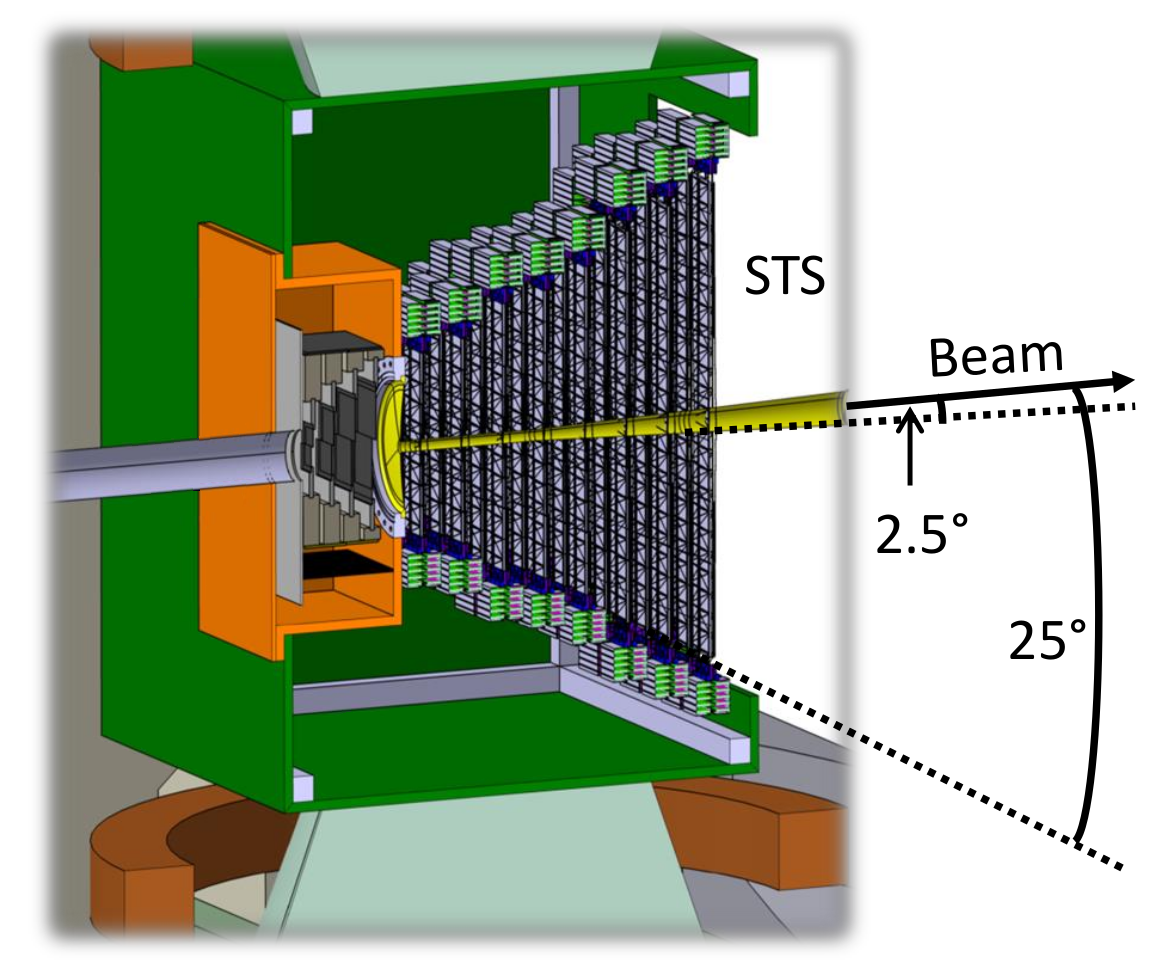
\includegraphics[width=0.8\textwidth]{pictures/STS_1.png}
%\end{minipage}
\caption{STS внутри термоизолирующего контейнера (зелёная) между полюсами магнита рядом с вакуумной камерой (оранжевая).}
\label{fig:STS12}
\end{figure}

%\hspace{0.01\textwidth}
%\begin{minipage}[b]{0.495\textwidth}
%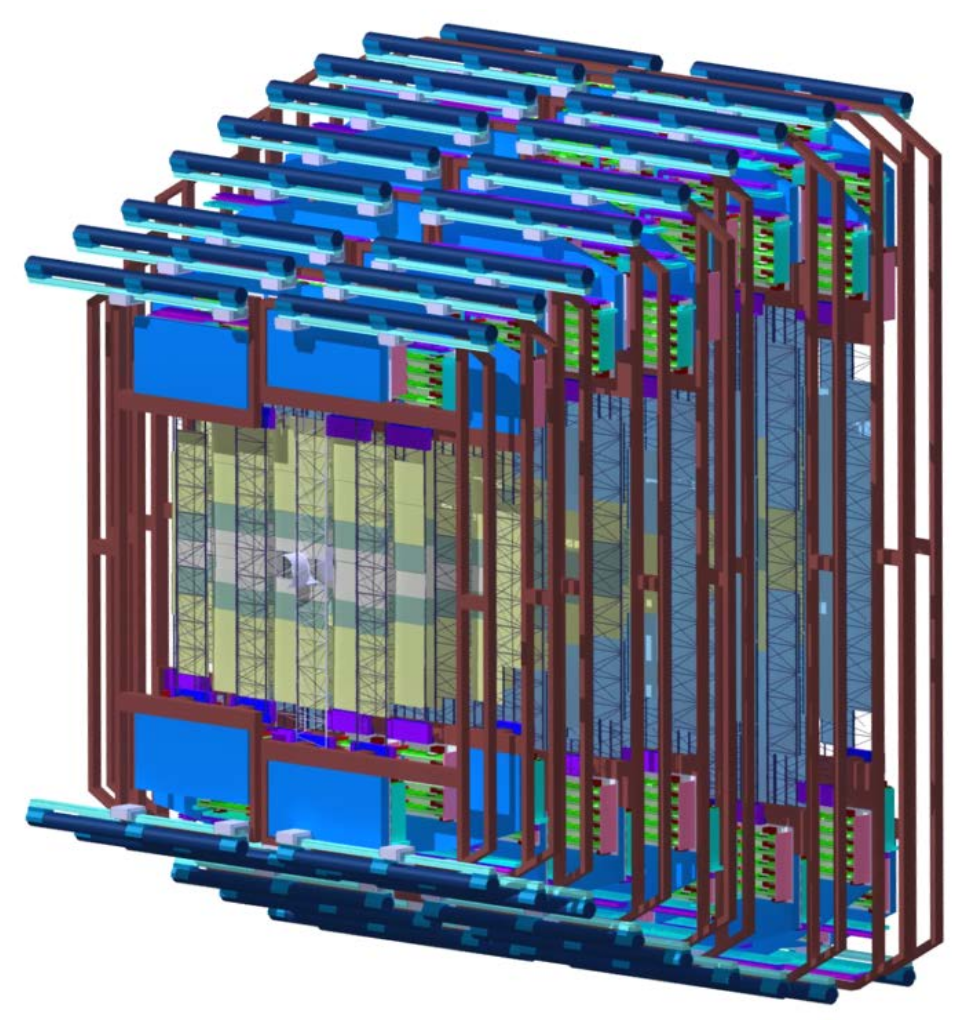
\includegraphics[width=1.0\textwidth]{pictures/STS_3.png}
%\end{minipage}

Считывание STS будет осуществляться специально разработанной электроникой, в основе которой лежит чип STS-XYTER. Он включает в себя 128~каналов, состоящих из зарядочувствительного усилителя, формирователя и 5-битного аналогово-цифрового преобразователя. На каждую зарегистрированную частицу каждый канал формирует временную отметку и значение АЦП, соответствующее оставленному заряду.

%\small{The chip includes 128 channels consisting of a charge sensitive amplifier (CSA), a shaper (SH) and an analogue to digital converter (ADC). For a particle hit, each channel provides the time stamp value and the ADC value corresponding to the deposited charge.}

%\begin{figure}[H]
%\centering
%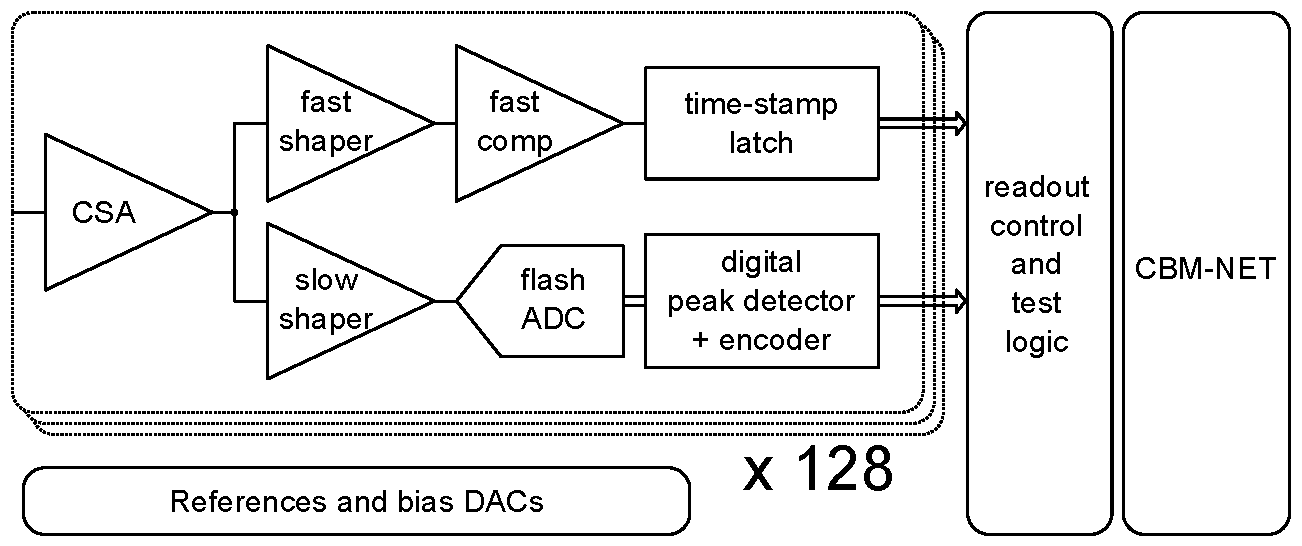
\includegraphics[width=0.95\textwidth]{pictures/STSXYTER.png}
%\caption{Блок-схема ПЛИС STS-XYTER.}
%\label{fig:STSXYTER}
%\end{figure}

%\todo
% Временные характеристики - оставить в каком-то виде?
%\textbf{Временное разрешение STS --- порядка 15~нс. Временное разрешение восстановленного хита как пересечения стрипов --- порядка 5~нс. Временное разрешение восстановленного трека, минимум по 4~станциям, --- порядка 1~нс. Время пролёта частицы через STS --- порядка 1~нс.}

% \subsubsection{Построение хита в STS}

STS --- главный трековый детектор эксперимента CBM. Частица, проходящая через двухстороний микростриповый сенсор, возбуждает сигналы в стрипах. Реконструкция треков по зарегистрированным в STS сигналам составляет значительную часть глобальной реконструкции и представляет собой сложную вычислительную задачу.

Первый этап реконструкции --- построение хита. Процедура поиска хитов определяет координаты $x$ и $y$ пролёта частицы через станцию по пересечению стрипов на двух сторонах сенсора. Координата $z$ фиксирована и определяется положением станции. Возможна ситуация, когда одна частица активирует кластер из двух или трёх рядом стоящих стрипов на одной стороне. В этом случае для определения пересечения используются усреднённые виртуальные стрипы. По сигналам с нескольких станций, расположенных на разных $z$, восстанавливается трек частицы. Применение стриповых детекторов имеет существенный недостаток --- в случае, если в одной станции были зарегистрированы несколько частиц, комбинаторным образом растёт количество ложных (fake) хитов.% (см.~\figref{fig:STSfakes}).

% \todo ссылку куда-нибудь? STS TDR?

% \begin{figure}[H]
% \begin{minipage}[b]{0.395\textwidth}
% 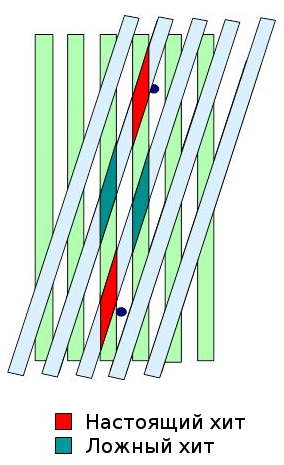
\includegraphics[width=0.95\textwidth]{pictures/Strip_detector.png}
% \end{minipage}
% \hspace{0.01\textwidth}
% \begin{minipage}[b]{0.495\textwidth}
% 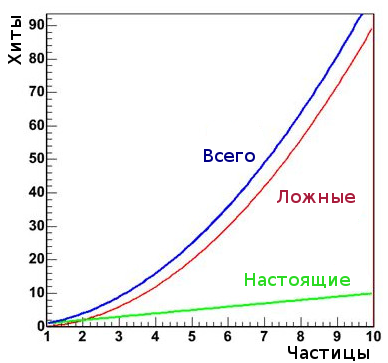
\includegraphics[width=0.95\textwidth]{pictures/Fake_hits.png}
% \end{minipage}
% \caption{Слева: две частицы зажигают 4 стрипа, что приводит к двум настоящим и двум ложным хитам. Справа: зависимость количества хитов от количества частиц.}
% \label{fig:STSfakes}
% \end{figure}

%\begin{minipage}[t]{0.495\textwidth}
%\begin{figure}[H]
%\centering
%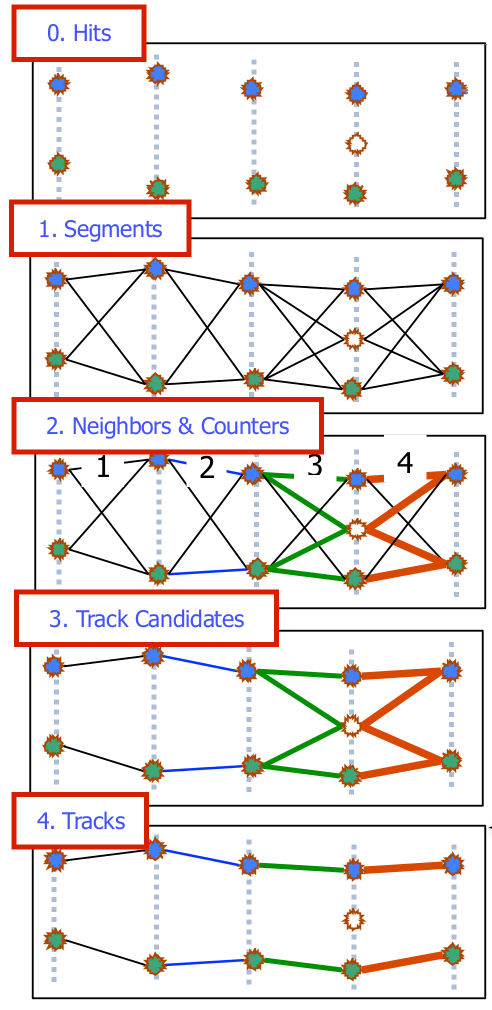
\includegraphics[width=0.95\textwidth]{pictures/Track_finding.png}
%\caption{Этапы алгоритма поиска треков в STS, основанном на клеточном автомате.}
%\label{fig:STStrackFinding}
%\end{figure}
%\end{minipage}
%\begin{minipage}[t]{0.495\textwidth}
Реконструкция треков в трековой системе STS осуществляется в два этапа --- поиск треков (track finding) и фитирование (track fitting).
%Поиск треков состоит из четырёх этапов, представленных на~\figref{fig:STStrackFinding}. \\
%Входная информация для поиска треков --- хиты, которые в случае стриповых детекторов получаются в результате выполнения процедуры поиска хитов. Первый этап поиска треков --- составление сегментов. На этом этапе строятся дуплеты и триплеты --- соответственно пары и тройки хитов на соседних станциях. Далее по смежным хитам определяются соседи. Затем составляются кандидаты треков. Хиты, вошедшие в кандидат трека выбрасываются из рассмотрения при построении следующих кандидатов. Из кандидатов выбираются результирующие треки. \\
Помимо ложных хитов, которые не соответствуют никаким реальным частицам, задача поиска треков в STS осложняется высоким фоном от дельта- и конверсионных электронов, рождённых на материале детектора.
Многократное рассеяние в материале приводит к изменению траекторий частиц.
Подробная геометрическая модель необходима для выполнения моделирования прохождения частиц через материал с учётом этих физических явлений с целью оптимизации алгоритмов трекинга.
%\end{minipage}

% ==========================================================================================================================
%__/\\\\____________/\\\\_____/\\\\\\\\\________/\\\\\\\\\\\\__/\\\\\_____/\\\__/\\\\\\\\\\\\\\\__/\\\\\\\\\\\\\\\_        
% _\/\\\\\\________/\\\\\\___/\\\\\\\\\\\\\____/\\\//////////__\/\\\\\\___\/\\\_\/\\\///////////__\///////\\\/////__       
%  _\/\\\//\\\____/\\\//\\\__/\\\/////////\\\__/\\\_____________\/\\\/\\\__\/\\\_\/\\\___________________\/\\\_______      
%   _\/\\\\///\\\/\\\/_\/\\\_\/\\\_______\/\\\_\/\\\____/\\\\\\\_\/\\\//\\\_\/\\\_\/\\\\\\\\\\\___________\/\\\_______     
%    _\/\\\__\///\\\/___\/\\\_\/\\\\\\\\\\\\\\\_\/\\\___\/////\\\_\/\\\\//\\\\/\\\_\/\\\///////____________\/\\\_______    
%     _\/\\\____\///_____\/\\\_\/\\\/////////\\\_\/\\\_______\/\\\_\/\\\_\//\\\/\\\_\/\\\___________________\/\\\_______   
%      _\/\\\_____________\/\\\_\/\\\_______\/\\\_\/\\\_______\/\\\_\/\\\__\//\\\\\\_\/\\\___________________\/\\\_______  
%       _\/\\\_____________\/\\\_\/\\\_______\/\\\_\//\\\\\\\\\\\\/__\/\\\___\//\\\\\_\/\\\\\\\\\\\\\\\_______\/\\\_______ 
%        _\///______________\///__\///________\///___\////////////____\///_____\/////__\///////////////________\///________
% ==========================================================================================================================

\subsection{Дипольный магнит}\label{sec:secMagnet}

Основная задача магнита --- искривлять траектории заряженных частиц, что позволит определять их импульс по радиусу кривизны после реконструкции в STS. Также магнитное поле разводит заряженные частицы в пространстве для уменьшения их плотности. Для решения указанных задач магнит должен создавать максимально равномерное стационарное вертикальное магнитное поле в заданной области пространства, а также минимизировать поле за пределами этой области.
% Это даёт возможность их регистрации детекторами, стоящими как внутри, так и ниже по пучку.

В CBM принято решение использовать Н-образный магнит с двумя сверхпроводящими круговыми обмотками, обеспечивающими интеграл поля 1~Тл$\cdot$м. Обмотки будут выполнены из NbTi, намотаны на цилиндрическую бобину и будут иметь два контура охлаждения жидким гелием --- при температуре $4.5K$ и $50K$.
Интеграл поля по всей области, где находится STS: 0.972~Тл$\cdot$м, макс. поле $\approx$~1~Тл. Отклонение интеграла поля по всему телесному углу по прямым линиям не превышает~10\%.
Геометрия магнита (см.~\figref{fig:MagnetDrawing}) определяется геометрическим аксептансом эксперимента ($\pm \SI{25}{\degree}$ по вертикали и $\pm \SI{30}{\degree}$ по горизонтали.) и тем фактом, что мишень, вершинный микродетектор MVD и кремниевая трековая система STS должны располагаться внутри магнитного поля.

Магнит должен иметь способность переключать полярность.
На поверхности магнита имеются съёмные магнитные экраны, используемые при работе с детектором черенковских колец. %field clamps
Конструкция магнита должна подразумевать сборку на месте.
Внутри магнита размещается термоизолированный контейнер, содержащий вакуумную камеру, MVD, STS и STS-секцию ионопровода длиной примерно 1.2~м. Эта секция подключается к следующей секциии ионопровода через разъёмное соединение. Для обслуживания оборудования контейнер как целое извлекается из магнита вверх по пучку.

\begin{figure}[H]
\centering
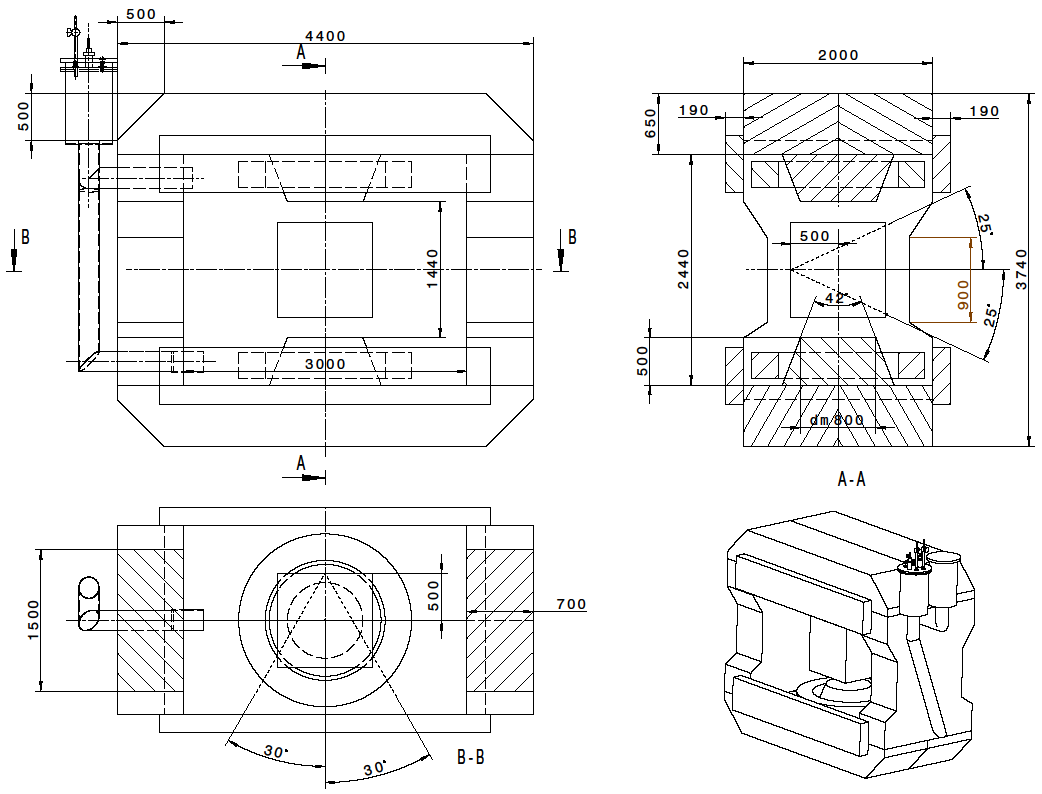
\includegraphics[width=0.7\textwidth]{pictures/Magnet_drawing.png}
\caption{Чертёж магнита.} % из CBM Dipole Detailed Specification из Collaboration Contract between the FAIR GmbH and BINP
\label{fig:MagnetDrawing}
\end{figure}

%\begin{figure}[H]
%\centering
%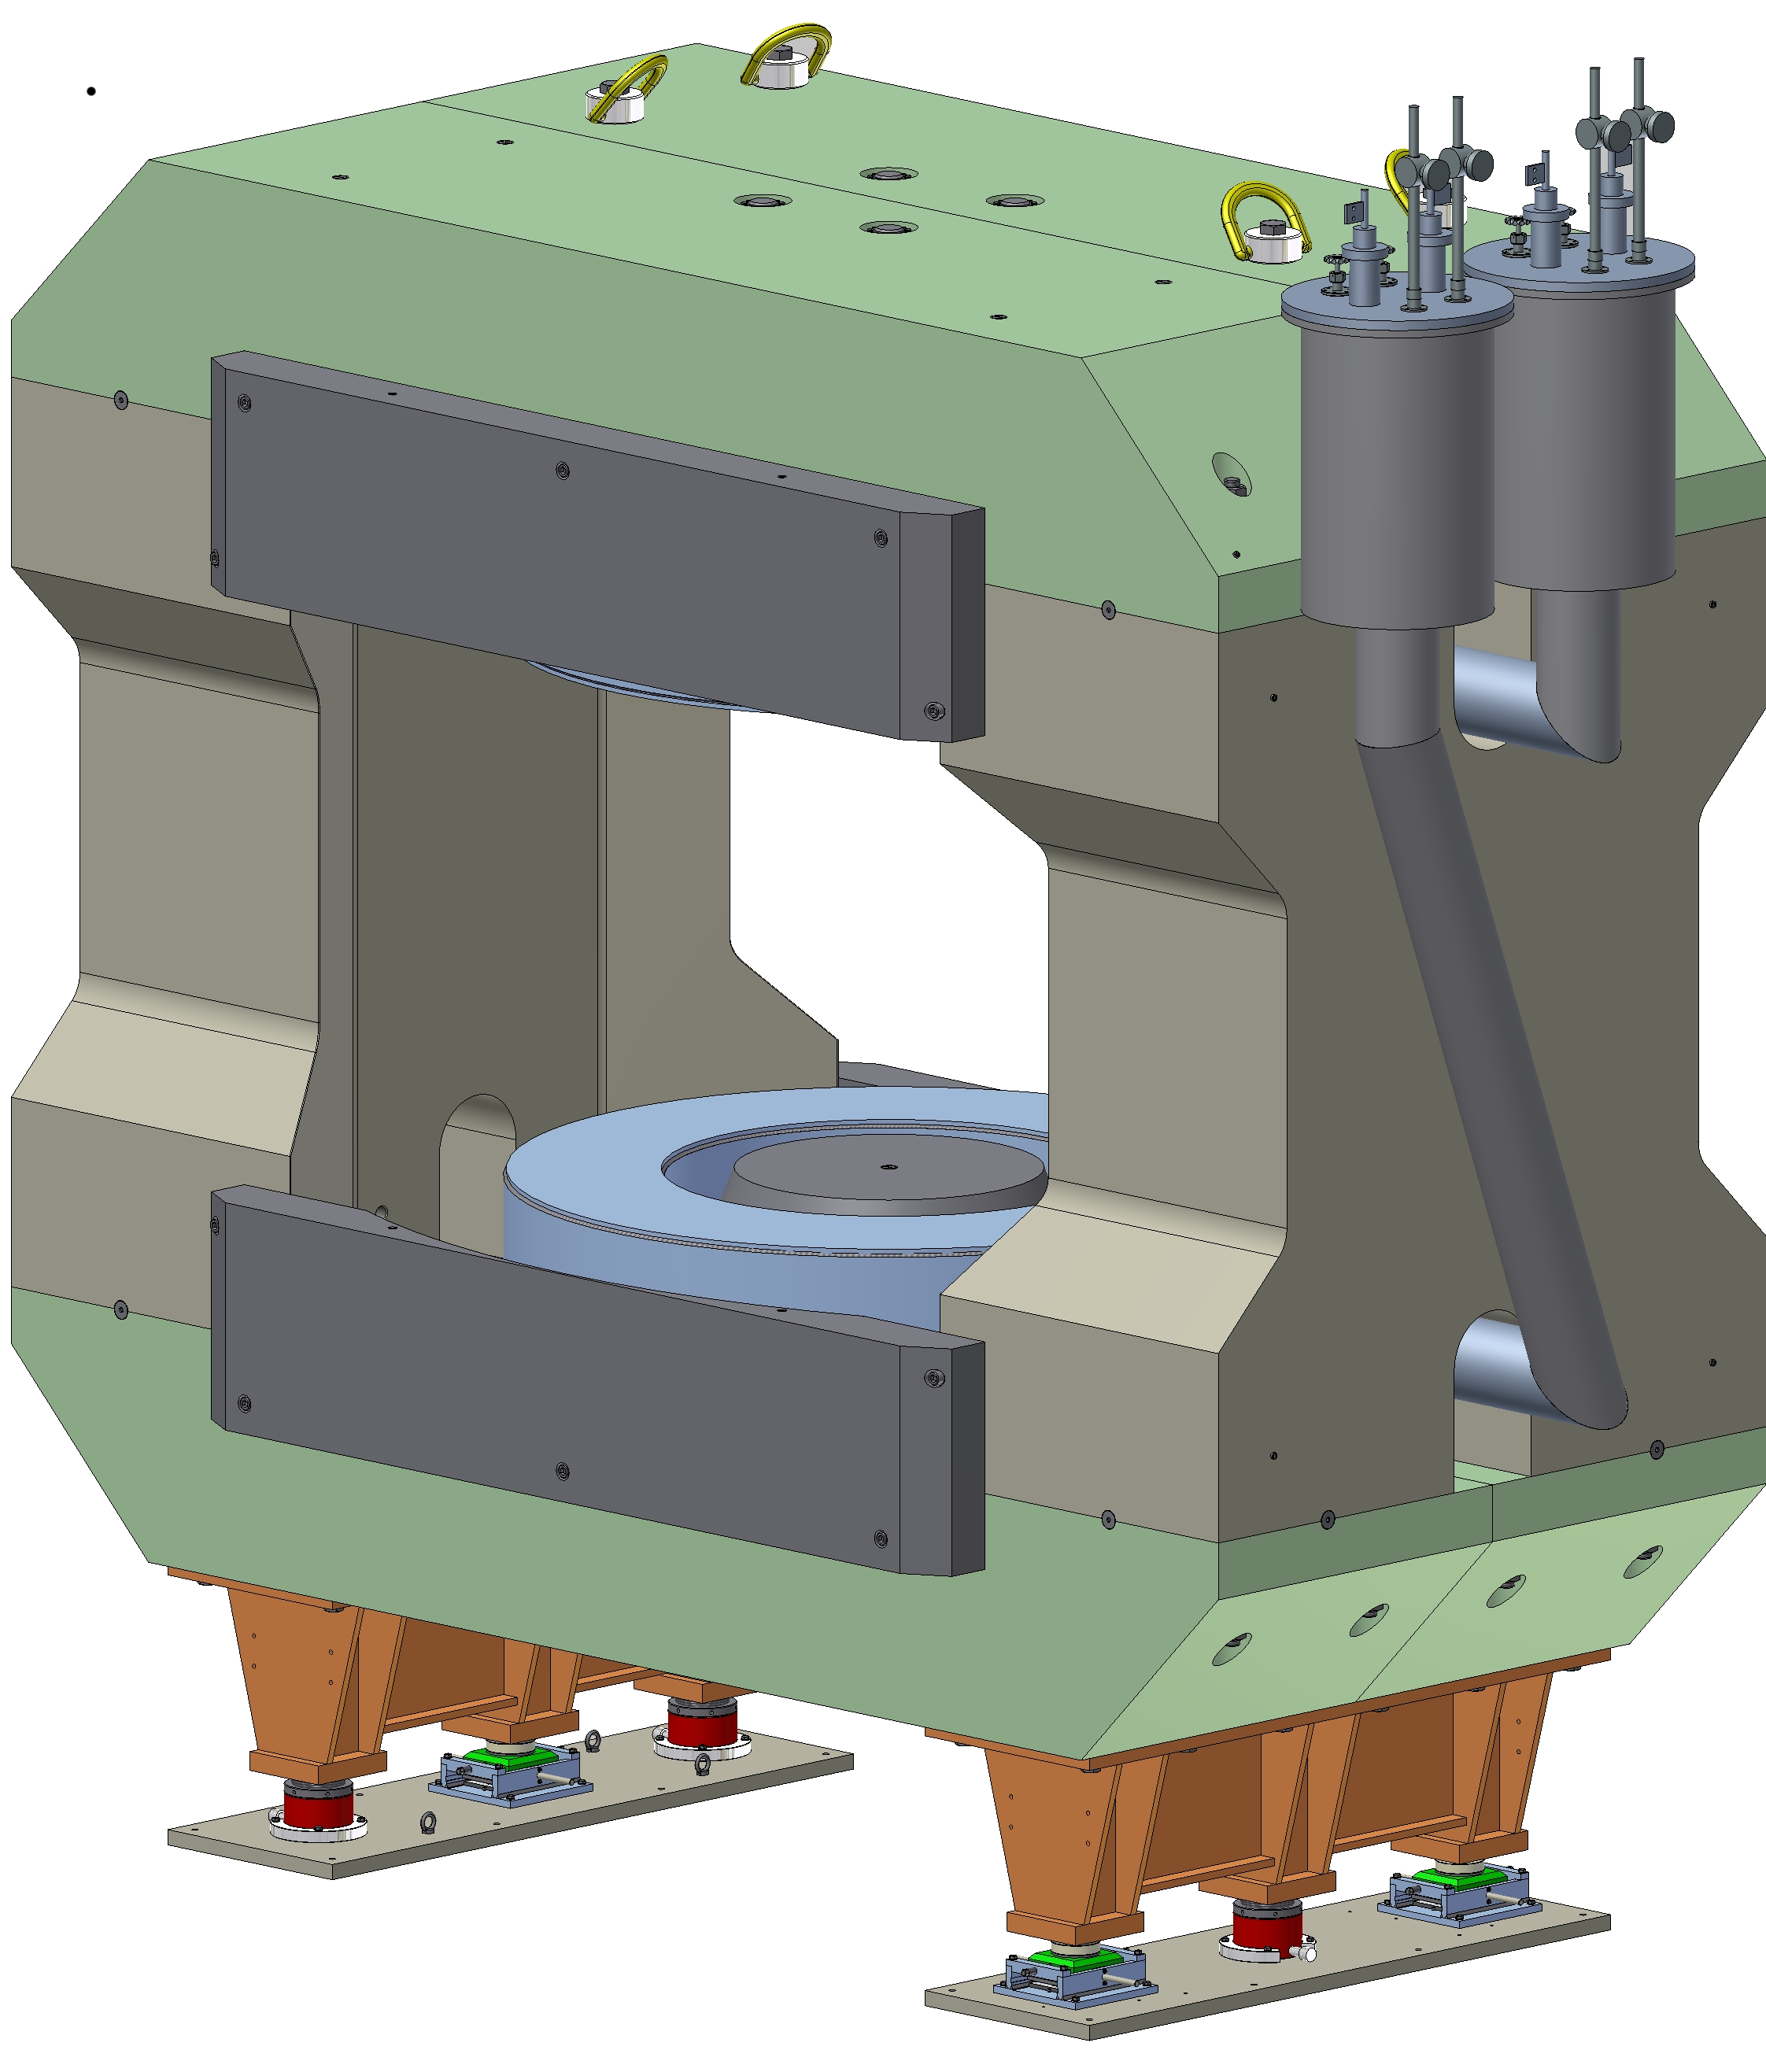
\includegraphics[width=0.7\textwidth]{pictures/CBM_magnet_model.png}
%\caption{Модель магнита}
%\label{fig:MagnetModel}
%\end{figure}

% ==========================================================================================================================
%____/\\\\\\\\\______/\\\\\\\\\\\________/\\\\\\\\\__/\\\________/\\\_        
% __/\\\///////\\\___\/////\\\///______/\\\////////__\/\\\_______\/\\\_       
%  _\/\\\_____\/\\\_______\/\\\_______/\\\/___________\/\\\_______\/\\\_      
%   _\/\\\\\\\\\\\/________\/\\\______/\\\_____________\/\\\\\\\\\\\\\\\_     
%    _\/\\\//////\\\________\/\\\_____\/\\\_____________\/\\\/////////\\\_    
%     _\/\\\____\//\\\_______\/\\\_____\//\\\____________\/\\\_______\/\\\_   
%      _\/\\\_____\//\\\______\/\\\______\///\\\__________\/\\\_______\/\\\_  
%       _\/\\\______\//\\\__/\\\\\\\\\\\____\////\\\\\\\\\_\/\\\_______\/\\\_ 
%        _\///________\///__\///////////________\/////////__\///________\///__
% ==========================================================================================================================

\subsection{Детектор черенковских колец RICH}\label{sec:secRICH}

Детектор черенковских колец (Ring Imaging CHerenkov detector, RICH) решает задачу идентификации электронов в диапазоне импульсов от 0.5~\GeVoverC{} до 8~\GeVoverC{}.
В паре с детектором переходного излучения TRD, стоящем ниже по пучку и покрывающем более высокие импульсы, RICH позволяет идентифицировать электроны от лёгких векторных мезонов, $J/\psi$ и $\psi'$-частиц, выделяя их из огромного потока $\pi$-мезонов.

Фактор подавления $\pi$-мезонов $\pi_{suppr}$ определяется как отношение количества восстановленных в STS треков $\pi$-мезонов, имеющих продолжение в геометрическом аксептансе детектора RICH, к количеству $\pi$-мезонов, идентифицированных как электроны.

Для получения дилептонных спектров на SIS300 требуется $\pi_{suppr}$ порядка 10000, что осуществимо при совместном применении TRD и RICH, причём $\pi_{suppr}$ последнего должен составлять как минимум 100.

По той причине, что в столкновении тяжёлых ионов рождается огромное количество заряженных $\pi$-мезонов, возникает необходимость идентифицировать электроны и позитроны.

\textbf{Переработать от ----------------------------------}

В случае SIS100 фон обусловлен такими источниками как $\gamma$-конверсия в мишени или распад $\pi^{0} \rightarrow \gamma + e^{+} + e^{-}$.

CBM RICH предсталяет собой классический RICH-детектор с газовым радиатором, с одним сферическим зеркалом и МА~ФЭУ в качестве фотодетекторов.

CBM RICH имеет $CO_{2}$ радиатор, который характеризуется коэффициентом преломления $n=1.00045$ при $T=0$ и $p=1$ атм.

\textbf{Переработать до ----------------------------------}

Более подробно CBM RICH рассмотрен в секции~\ref{sec:secCBMrich}.

% ==========================================================================================================================
%__/\\\\____________/\\\\__/\\\________/\\\________/\\\\\\\\\__/\\\________/\\\_        
% _\/\\\\\\________/\\\\\\_\/\\\_______\/\\\_____/\\\////////__\/\\\_______\/\\\_       
%  _\/\\\//\\\____/\\\//\\\_\/\\\_______\/\\\___/\\\/___________\/\\\_______\/\\\_      
%   _\/\\\\///\\\/\\\/_\/\\\_\/\\\_______\/\\\__/\\\_____________\/\\\\\\\\\\\\\\\_     
%    _\/\\\__\///\\\/___\/\\\_\/\\\_______\/\\\_\/\\\_____________\/\\\/////////\\\_    
%     _\/\\\____\///_____\/\\\_\/\\\_______\/\\\_\//\\\____________\/\\\_______\/\\\_   
%      _\/\\\_____________\/\\\_\//\\\______/\\\___\///\\\__________\/\\\_______\/\\\_  
%       _\/\\\_____________\/\\\__\///\\\\\\\\\/______\////\\\\\\\\\_\/\\\_______\/\\\_ 
%        _\///______________\///_____\/////////___________\/////////__\///________\///__
% ==========================================================================================================================

\subsection{Мюонная система MUCH}\label{sec:secMUCH}

% From CBM MUCH TDR:

% ссылка на картинку fig:MUCH2

\begin{minipage}[b]{0.495\textwidth}
Мюонная система (MUon CHambers, MUCH) необходима для идентификации мюонных пар, на которые распадаются лёгкие векторные мезоны и частицы со скрытым очарованием.
%рождённых в высокоэнергетичных столкновениях тяжёлых ионов в диапазоне энергий пучка от~4~до~40~\GeVperNucl{}. Измерение лептонных пар является одним из центральных пунктов физической программы CBM, так как они несут информацию о состоянии материи внутри фаербола. В области низких инвариантных масс дилептоны предоставляют информацию о модификации векторных мезонов в среде, что является многообещающей наблюдаемой о восстановлении киральной симметрии. В области средних инвариантных масс в спектре дилептонов преобладает termal \todo радиация от фаербола, которая говорит о его температуре. В области инвариантных масс около 3~\GeVoverC{}$^{2}$ дилептоны представляют собой подходящий инструмент для изучения аномального подавления чармония в фазе деконфайнмента. В эксперименте CBM для получения полной картины о дилептонной физике будут измеряться как электроны, так и мюоны.
Основной сложностью при измерении мюонов в столкновениях тяжёлых ионов при энергиях пучка, предоставляемых FAIR, является идентификация мюонов с низким импульсом в среде с очень высокой плотностью частиц. Стратегия, выбранная CBM, заключается в том, чтобы выполнять трекинг в системе с адронными абсорберами и выполнять идентификацию мюонов в зависимости от импульса. По этой причине мюонная система будет выполнена в виде последовательности адронных абсорберов и тройных трековых станций. Адронные абсорберы различаются по толщине и материалу, а трековые станции, в зависимости от требуемой гранулярности, состоят из детекторов, выполненных по технологиям GEM и Micromegas, предоставляющих пространственное разрешение порядка 50~мкм, а также straw tubes, обеспечивающих разрешение порядка 100~мкм. В качестве последней трековой станции будет использоваться станция детектора TRD. MUCH будет расположен за дипольным магнитом, в том же месте, где стоит RICH в электронной конфигурации CBM. Чтобы уменьшить количество мюонов от слабых распадов $\pi$-мезонов и $K$-мезонов, система из абсорберов и детекторов должна быть максимально компактна. % \todo проверить формулировку про разрешение
\end{minipage}
\begin{minipage}[b]{0.495\textwidth}
\begin{figure}[H]
\centering
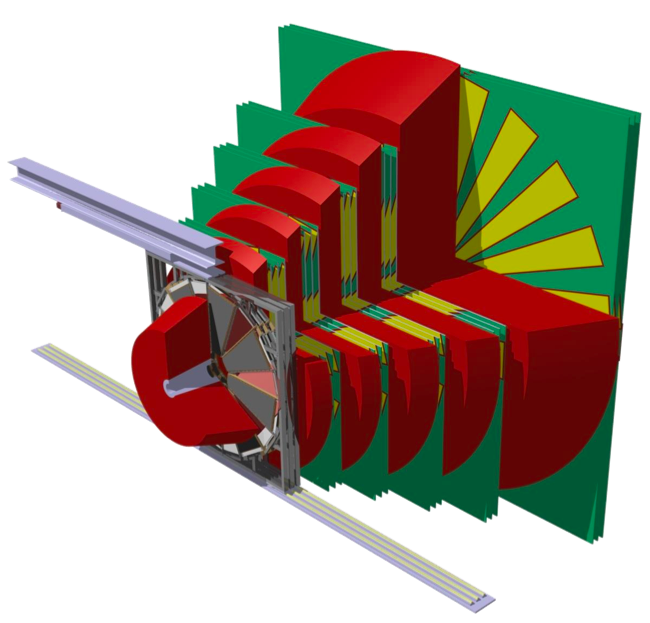
\includegraphics[width=0.95\textwidth]{pictures/CBM_MUCH_model.png}
\caption{Модель мюонной системы MUCH. Красным цветом показаны абсорберы, газовые детекторы --- жёлтым, опоры --- зелёным.}
\label{fig:MUCH2}
\end{figure}
\end{minipage}

% The first two stations will consist of triple Gas Electron Multiplier (GEM) detectors, and the next one or two stations will be made of straw tube detectors. As the last tracking station behind the thick 1m absorber we use four layers of the Transition Radiation Detector (TRD) which is built for electron identification at CBM.

% http://localhost/Lib/much-tdr-final-for-gsi-report.pdf
% таблица, страница 30
% страница 130

Считывание детекторов, изготовленных по технологии GEM и Micromegas, будет осуществляться платами на основе специального чипа, аналогичного STS-XYTER, разрабатываемого для кремниевой трековой системы. Считывание straw tubes --- платами передней электроники PADI, разрабатываемыми для время-пролётного детектора.

%\small{The MuCh system is designed to identify muon pairs which are produced in high-energy heavy-ion collisions in the beam energy range from~4~to~40~AGeV. The measurement of lepton pairs is a central part of the CBM research program, as they are very sensitive diagnostic probes of the conditions inside the fireball. At low invariant masses, dileptons provide information on the in-medium modification of vector mesons which is a promising observable for the restoration of chiral symmetry. At intermediate invariant masses, the dilepton spectrum is dominated by thermal radiation from the fireball reflecting its temperature. At invariant masses around $ 3 GeV/c^{2} $, dileptons are the appropriate tool to study the anomalous charmonium suppression in the deconfined phase. In the CBM experiment both electrons and muons will be measured in order to obtain a consistent and comprehensive picture of the dilepton physics.}

% перенёс абзац внутрь minipage

%\small{The experimental challenge for muon measurements in heavy-ion collisions at FAIR energies is to identify low-momentum muons in an environment of high particle densities. The CBM strategy is to track the particles through a hadron absorber system, and to perform a momentum-dependent muon identification. This concept is realized by an instrumented hadron absorber, consisting of staggered absorber plates and tracking stations. The hadron absorbers vary in material and thickness, and the tracking stations consist of detector triplets based on different technologies. The MuCh system is placed downstream of the dipole magnet hosting the Silicon Tracking System (STS) which determines the particle momentum. In order to reduce the number of muons from pion and kaon weak decays, the absorber/detector system has to be as compact as possible.}

Мюонная система будет строиться поэтапно соответственно энергиям пучка, предоставляемым ускорителем.
%В рамках FAIR MSV (\todo ссылка) синхротрон SIS100 будет выдавать пучок тяжёлых ионов с энергией до 14~\GeVperNucl{} и протонный пучок с энергией до 29~\GeVperNucl{}.
Две первые версии MUCH (SIS100-A и SIS100-B) будут состоять из~3~и~4~станций соответственно, что подходит для измерения лёгких векторных мезонов в столкновениях при 4--6~\GeVperNucl{} и 8--14~\GeVperNucl{} соответственно. Третья версия MUCH (SIS100-C) будет оборудована дополнительным железным абсорбером толщиной 1~м для того, чтобы идентифицировать чармоний при самых высоких энергиях SIS100.
По введении в эксплуатацию SIS300 мюонная система будет обновлена введением дополнительной станции абсорера и детектора для измерения лёгких векторных мезонов и чармония при энергиях пучка более 14~\GeVperNucl{} (версии SIS300-A и SIS300-B).

%\small{The MuCh system will be built in stages which are adapted to the beam energies available. Within the FAIR modularized start version the SIS100 ring will provide heavy ion beams with energies up to 14~AGeV, and proton beams up to 29~GeV. The first two versions of MuCh (SIS100-A and SIS100-B) will comprise of~3~and~4 stations suitable for the measurement of low-mass vector mesons in $ A + A $ collisions at 4-6~AGeV and 8-14~AGeV, respectively. The third version of the MuCh system (SIS100-C) will be equipped with an additional iron absorber of 1~m thickness in order to be able to identify charmonium at the highest SIS100 energies.}

%\small{The absorber slices will be built only once so that they could be rearranged properly to obtain required absorber thicknesses. Once SIS300 is operational, we will upgrade the MuCh system further by inserting additional absorbers and detector stations for the measurement of low-mass vector mesons and charmonium at beam energies above 14~AGeV (MuCh versions SIS300-A and SIS300-B).}

%\begin{figure}[H]
%\centering
%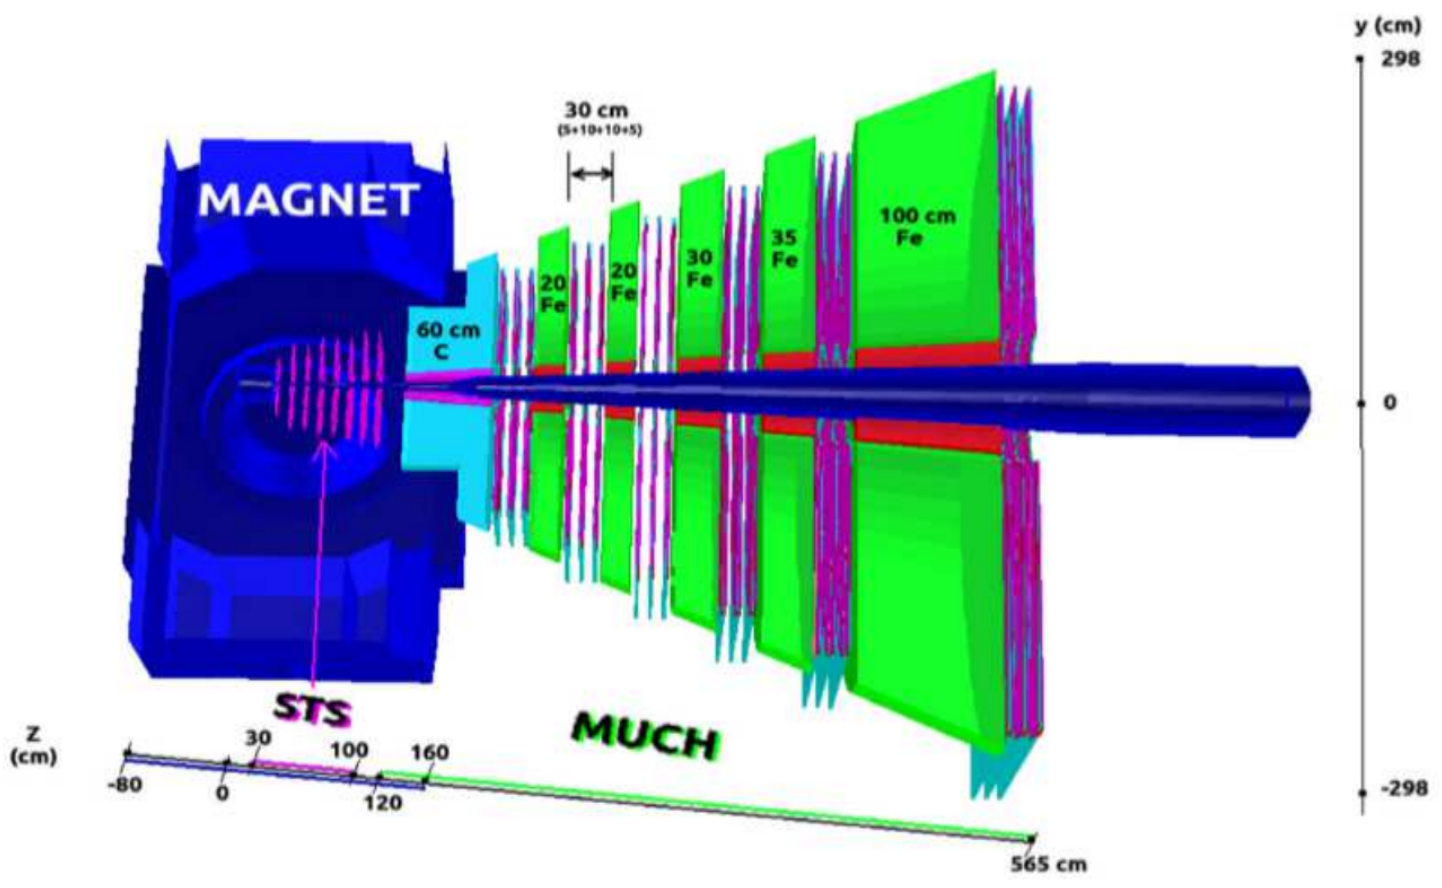
\includegraphics[width=1.0\textwidth]{pictures/MUCH.png}
%\caption{Схема расположения станций мюонной системы.}
%\label{fig:MUCH}
%\end{figure}

% ==========================================================================================================================
%__/\\\\\\\\\\\\\\\____/\\\\\\\\\______/\\\\\\\\\\\\____        
% _\///////\\\/////___/\\\///////\\\___\/\\\////////\\\__       
%  _______\/\\\_______\/\\\_____\/\\\___\/\\\______\//\\\_      
%   _______\/\\\_______\/\\\\\\\\\\\/____\/\\\_______\/\\\_     
%    _______\/\\\_______\/\\\//////\\\____\/\\\_______\/\\\_    
%     _______\/\\\_______\/\\\____\//\\\___\/\\\_______\/\\\_   
%      _______\/\\\_______\/\\\_____\//\\\__\/\\\_______/\\\__  
%       _______\/\\\_______\/\\\______\//\\\_\/\\\\\\\\\\\\/___ 
%        _______\///________\///________\///__\////////////_____
% ==========================================================================================================================

\subsection{Детектор переходного излучения TRD}\label{sec:secTRD}

% Радиатор и spadic

Основная задача детектора переходного излучения (Transition Radiation Detector, TRD) --- идентифицировать электроны с импульсом более 1~\GeVoverC{} для того чтобы расширить возможности детектора RICH по идентификации частиц в диапазоне импульсов около 5~\GeVoverC{}.
Такая идентификация должна быть достигнута при коэффициенте подавления $\pi$-мезонов порядка 10--20 для получения возможности измерения диэлектронов в диапазоне масс от $\rho$ до $\psi'$.
Благодаря способности идентифицировать заряженные частицы за счёт их известного энерговыделения детектор TRD также предоставит ценную информацию при регистрации лёгких ядерных осколков.
Это особенно важно для отделения, например, дейтронов от $ ^{4}He $, которое не может быть достигнуто с помощью одного только детектора TOF.

%\small{The main task of the TRD is to identify electrons above momenta of 1 GeV/c and thus to extend the electron identification capabilities of the Ring Image CHerenkov (RICH) detector above momenta of p $\approx$ 5 GeV/c. This identification has to be achieved with a pion suppression factor in the range 10--20, in order to allow for a measurement of dielectrons in the mass range from below the $\rho$ and $\omega$ masses to beyond the $J/\psi$ mass with a good signal-to-background ratio. Due its capability to identify charged particles via their specific energy loss, the TRD in addition will provide valuable information for the measurement of nuclear fragments. This is in particular important for the separation of, e.g, deuterons and $ ^{4}He $, which cannot be achieved using a time-of-flight measurement alone.}

Указанные требования могут быть удовлетворены применением многопроволочных пропорциональных камер (MWPC) на основе $ Xe/CO_{2} $ в связке с подходящим радиатором. Базовая версия CBM TRD оснащена MWPC с симметричной зоной усиления толщиной 3.5~мм + 3.5~мм и далее областью дрейфа толщиной 5~мм, наличие которой увеличивает вероятность поглощения фотона переходного излучения в активном газовом объёме. Такая геометрия обеспечивает эффективное и быстрое формирование выходного сигнала
Высокая эффективность детектора достигается минимизацией материала между радиатором и газом.

%\small{These requirements can be fulfilled with Xe/CO 2 based Multi-Wire Proportional Chambers (MWPC) detector in combination with an adequate radiator. The default MWPC for the CBM-TRD is composed of a symmetric amplification area of 3.5 + 3.5 mm thickness, followed by a 5 mm drift region to enhance the TR-photon absorption probability in the active gas volume. This geometry provides also efficient and fast signal creation, as well as readout, with timescales below 200 $\mu$s per charged particle track. The performance of the detector is optimized by reducing the material budget between radiator and gas volume to a minimum.}

Базовая версия CBM TRD предполагает одну станцию, состоящую из четырёх слоёв. Она будет расположена между детекторами RICH и TOF. Помимо идентификации электронов в электронной конфигурации, станция детектора TRD будет использоваться в качестве последней трековой станции детектора MUCH в мюонной конфигурации. Отметим также, что наличие дополнительной станции между STS и TOF повышает качество реконструкции треков.

%\small{The baseline design of the TRD foresees one station composed of four detector layers. It will be positioned between the RICH and the Time-Of-Flight (TOF) detector and thus allows to reduce the background in the TOF resulting from track mismatches by providing additional position information for high precision tracking between Silicon Tracking System (STS) and TOF. The TRD will also be used as tracking station behind the last absorber of the MUCH detector in the muon configuration of CBM.}

Для считывания детектора переходного излучения разрабатывается специальный самотриггерующийся чип, называемый SPADIC (Self-triggered Pulse Amplification and Digitization). Он включает в себя логику формирования хита и оцифровку формы импульса (\cite{SPADIC}).

% ==========================================================================================================================
%__/\\\\\\\\\\\\\\\_______/\\\\\_______/\\\\\\\\\\\\\\\_        
% _\///////\\\/////______/\\\///\\\____\/\\\///////////__       
%  _______\/\\\_________/\\\/__\///\\\__\/\\\_____________      
%   _______\/\\\________/\\\______\//\\\_\/\\\\\\\\\\\_____     
%    _______\/\\\_______\/\\\_______\/\\\_\/\\\///////______    
%     _______\/\\\_______\//\\\______/\\\__\/\\\_____________   
%      _______\/\\\________\///\\\__/\\\____\/\\\_____________  
%       _______\/\\\__________\///\\\\\/_____\/\\\_____________ 
%        _______\///_____________\/////_______\///______________
% ==========================================================================================================================

\subsection{Время-пролётный детектор TOF}\label{sec:secTOF}

\textbf{В TDR есть неплохие картинки (см. стр 74).}

% From CBM TOF TDR:

Основная задача время-пролётного детектора (Time Of Flight detector, TOF) --- измерять момент времени прихода заряженных частиц, чтобы провести идентификацию после сопоставления хита TOF с соответствующим треком кремниевой трековой системы STS.

%\small{The detector system’s prime task is to measure the arrival time of charged particles to allow for their identification after having matched the TOF - hit with the corresponding STS track obtained from the CBM silicon tracking system (STS).}

%\small{Система для измерения времени пролёта возможна только при наличии детектора, регистрирующего момент старта --- временную отметку $T_{0}$ первичного взаимодействия.}
CBM TOF состоит из двух частей --- стартовый детектор (Start Detector, SD) в непосредственной близости к точки первичного взаимодействия и TOF-стена на подвижной опоре, располагаемая на расстоянии 6--10~м от мишени в зависимости от выполняемой программы измерений CBM. Быстродействующий алмазный стартовый детектор, расположенный на пучке, может удовлетворять всем требованиям CBM, включая полный диапазон пучка --- от протонов до тяжёлых ионов. Такой детектор в то же время может эффективно использоваться для онлайн диагностики пучка, мгновенно выдавая информацию о профиле пучка, стабильности его положения по отношению к мишени, о количестве частиц в гало и о временной структуре пучка. SD будет расположен внутри вакуумной камеры. Его толщина должна быть минимальна, чтобы минимизировать взаимодействие с пучком.

%\small{The proposal of a high performance TOF wall would be incomplete without the discussion of the time - zero (T 0 ) - reference that is needed for any velocity measurement. Details can be found in chapter 4 demonstrating that for all of the anticipated running scenarios solutions are available. For most of the heavy-ion reaction running at the initial SIS100 accelerator the software based T 0 - extraction is sufficient (see section 4.2). This method can be calibrated by making use of the diamond based start detector system developed for the HADES experiment (section 4.4) that is operational up to interaction rates of 100 kHz. A high rate in-beam start detector (SD) could fulfill all CBM $T_{0}$ requirements, covering whole range of beams from proton to heavy-ions. Such detector is at the same time intended to be used for the on-line beam monitoring, giving the instantaneous information about the beam profile, the stability of the beam position on target, the amount of halo particles and time structure of the beam. In our opinion the best solution for such detector is an in-beam diamond Start detector. SD will be installed inside the beam pipe in vacuum and it will measure the arrival time of every beam particle. In order to reduce the interactions in the SD itself its thickness has to be minimized. Fig. 4.4 shows the mounting of the planned SD system between the last focusing magnet in front of the cave and the focal point of the CBM detector.}

%Так как CBM представляет собой эксперимент с фиксированной мишенью, поток заряженных частиц сильно зависит от направления.
Стена TOF будет собрана из модулей различной гранулярности и выполненных с разными требованиями к допустимой частоте. Чтобы иметь достаточную степень разделения, особенно для идентификации заряженных каонов, необходимо расстояние до 10~м и временное разрешение порядка 80~пс, что приводит к требуемому размеру TOF около 12$\times$9~м$^2$. Чтобы достичь указанного временного разрешения детектор должен быть оборудован электроникой с гарантированным временным разрешением лучше 60~пс и эффективностью лучше 95\%.

%\small{Since CBM is operated in fixed target mode the flux of charged particles is strongly varying with the polar angle. A modular TOF wall is proposed whose elements, called modules in the following, are adapted to the granularity and rate requirements. To allow for sufficient separation power especially for the identification of charged kaons, distances of up to 10 m and a system time resolution of 80 ps are necessary leading to an overall size of the TOF - wall of approx. 12$\times$9 m2 . To achieve the overall time resolution this area needs to get instrumented with timing detectors with an intrinsic timing resolution better than 60 ps and an efficiency better than 95\%.}

Предлагается построить CBM TOF на основе современных многозазорных резистивных плоских пропорциональных камер (Multigap Resistive Plate Chambers, MRPC). Базовый элемент этого детектора --- пачка резистивных пластин из стекла или керамики, которые разделены тонким зазором с газом. При достаточно высоком электрическом поле электронные лавины развиваются однородно по поверхности и сигнал от них можно считывать через емкостную связь.
Данный тип детекторов способен работать на частоте порядка 25~кГц/см$^2$, что стало возможным благодаря разработке стекла с низким сопротивлением.

%\small{The TOF wall will be built on the basis of state-of-the-art Multigap Resistive Plate Chambers (MRPC). The basic element of this robust detector concept is a stack of resistive plates made out of glass or ceramics that are separated by thin gas gaps. At sufficiently high electric field strength avalanches are created in a very uniform manner and can be read out via capacitive coupling.}

%\small{---- As is demonstrated in chapters 7 this 10 - years old detector technology is well advanced by now, largely due to the effort of the CBM - TOF group, and offers the flexibility to cope with the high demands posed by the CBM physics goals.}

%\small{Most notably, the proposed concept that requires a detector technology with a sustained rate capability in the order of 25 kHz/cm 2 became possible only by the development of a low - resistivity glass (see section 7.1.1) that is available for CBM - TOF by now through the CBM - TOF group at Tsinghua University, Beijing, China at reasonable costs.}

%\small{The proposed structure of the CBM - TOF wall is based on detector layouts that have already been realized and tested in in-beam experiments and demonstrated MRPC counter timing resolutions below 60 ps with efficiencies above 95\% at rates relevant for CBM (see chapter 7 for details). The basic element of the proposed wall are MRPC strip counters where a single avalanche is generating two signals at the two ends of a readout-electrode. The length of the readout - strip can be easily adjusted to the required granularity. The leading design goal of the proposed strip structures is operation stability and signal integrity. This is achieved by differential signal processing and the matching of the readout strip impedance to the input impedance of the newly developed preamplifier discriminator chip (PADI). Thus the number of spurious hits due to reflections is minimized and an optimal response of the detectors is guaranteed with minimal dead time. This aspect is considered to be especially important for the high rate running conditions of CBM where even independent events will be overlapping in time space and any additional spurious hit will deteriorate the system performance.}

CBM TOF будет собран из MRPC счётчиков четырёх типов, организованных в модули шести типов.
Счётчики отличаются типом резистивного стекла, количеством и шириной зазоров, и размером электродов. Ячейки варьируются от 4.7~см$^2$ до 53~см$^2$.

Для считывания время-пролётного детектора разрабатывается специальная плата предусилитель-дискриминатор PADI, сигнал с которой оцифровывается самотриггерующимся многоканальным ВЦП на основе ППВМ (FPGA) (\cite{PADI}).

%\small{The high performance electronics for the whole CBM - TOF wall is independent of the choice of a specific module or counter type and is based on the PADI and the GET4 - ASIC chips developed by the CBM--TOF group (see sections 3.3.3 and 3.3.5). The combination of both chips in conjunction with a custom-designed clock distribution system (section 3.3.8) offers the possibility to build a large scale system with an electronics contribution to the timing resolution of about 30 ps. This system was tested using a readout controller that implements the full CBMnet - protocol and allows for online inspection and control of the GET4 - data. The details of the readout-chain are described in section 3.3. However, since up to now no long - term stably working GET4 - system could be demonstrated, an alternative backup solution is also included in this report. It is built on FPGA based TDCs that became available recently (see appendix G.2) and provides timing resolution on the level of 10 ps. A free-streaming readout chain is not yet available, but is planned to be realized in the near future. As a consequence the number of necessary readout controllers would be substantially reduced leading eventually to a more simple and cost effective system. More R'n'D is required in the direction of an FPGA - based digitizer / readout system, specifically considering the radiation environment (see chapter 2.5). Since FPGA - based digitizers are offering a better resolution and more flexibility and would allow e.g. for an improvement of the double hit recognition the decision about the production of the GET4 - system will be taken only after a) the stability of the GET4 readout chain is proven, b) no competitive FPGA based solution is available until start of mass production (Dec.2015). Therefore R'n'D work on FPGA-based TDCs is continuing as part of the project.}

%\small{As has been shown by Monte-Carlo simulations using the SHIELD event generator the quality of the T 0 - reference determination can be improved by installing the so called Beam Fragmentation T 0 Counter (BFTC) as the innermost part of the TOF wall (see section 4.3). It should cover the region from about 20 to 60 cm from the beam pipe (overlapping with the PSD acceptance). Using a very simple algorithm without tracking information a T 0 - signal with a precision of better than 50 ps can be achieved. A detector concept, anticipated to be able to operate in this harsh environment with fluxes being as high as 100 kHz/cm 2 , built from very radiation-hard materials and possessing minimum gas aging characteristics, is suggested to be based on the ceramic electrodes (see section F.1). Single cell pads with the size of 2$\times$2 cm 2 seem to fulfill the double hit, maximum rate and cross-talks requirements. Further R'n'D is necessary in order to prove the validity of the concept.}

%\small{The very large dynamical range in terms of incident beam energies that has to be covered by the CBM experiment reflects itself by the movable wall concept where the whole TOF - system is mounted on rails and can be placed at various distances. The rail system is sketched in section 5.1. It allows e.g. to balance the decay losses for kaons against the purity of an anticipated online kaon multiplicity selection. It also enables the servicing of the components independently from the other subsystems of CBM during shutdown periods.}

\begin{figure}[H]
\centering
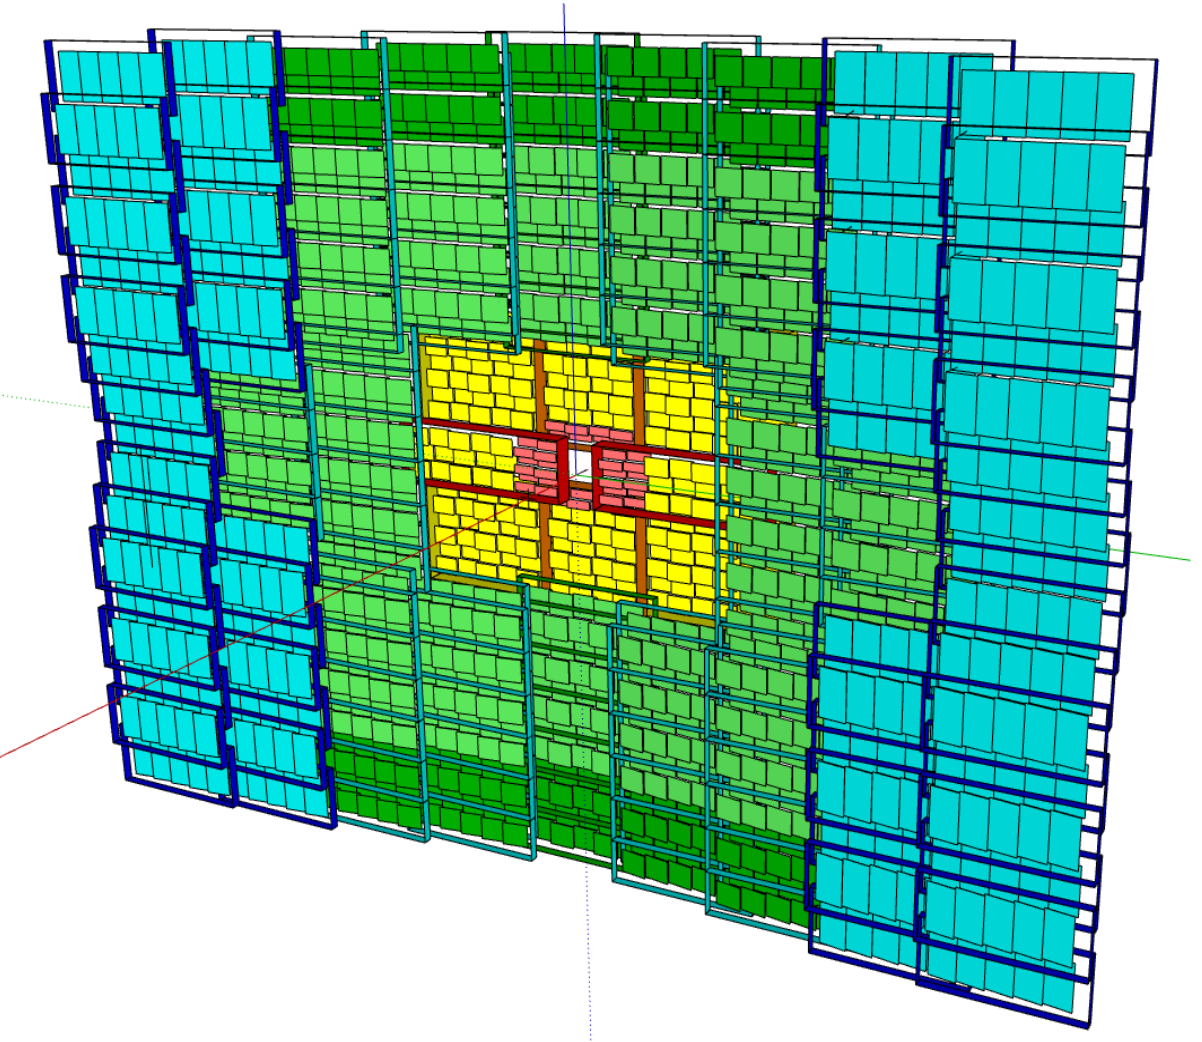
\includegraphics[width=0.6\textwidth]{pictures/TOF.png}
\caption{Модель стены время-пролётного детектора TOF.}
\label{fig:TOF}
\end{figure}

% ==========================================================================================================================
%__/\\\\\\\\\\\\\\\________/\\\\\\\\\_____/\\\\\\\\\_____/\\\_____________        
% _\/\\\///////////______/\\\////////____/\\\\\\\\\\\\\__\/\\\_____________       
%  _\/\\\_______________/\\\/____________/\\\/////////\\\_\/\\\_____________      
%   _\/\\\\\\\\\\\______/\\\_____________\/\\\_______\/\\\_\/\\\_____________     
%    _\/\\\///////______\/\\\_____________\/\\\\\\\\\\\\\\\_\/\\\_____________    
%     _\/\\\_____________\//\\\____________\/\\\/////////\\\_\/\\\_____________   
%      _\/\\\______________\///\\\__________\/\\\_______\/\\\_\/\\\_____________  
%       _\/\\\\\\\\\\\\\\\____\////\\\\\\\\\_\/\\\_______\/\\\_\/\\\\\\\\\\\\\\\_ 
%        _\///////////////________\/////////__\///________\///__\///////////////__
% ==========================================================================================================================

\subsection{Электромагнитный калориметр ECAL}\label{sec:secECAL}

% From CBM ECAL TDR

\begin{minipage}[t]{0.495\textwidth}
\begin{figure}[H]
\centering
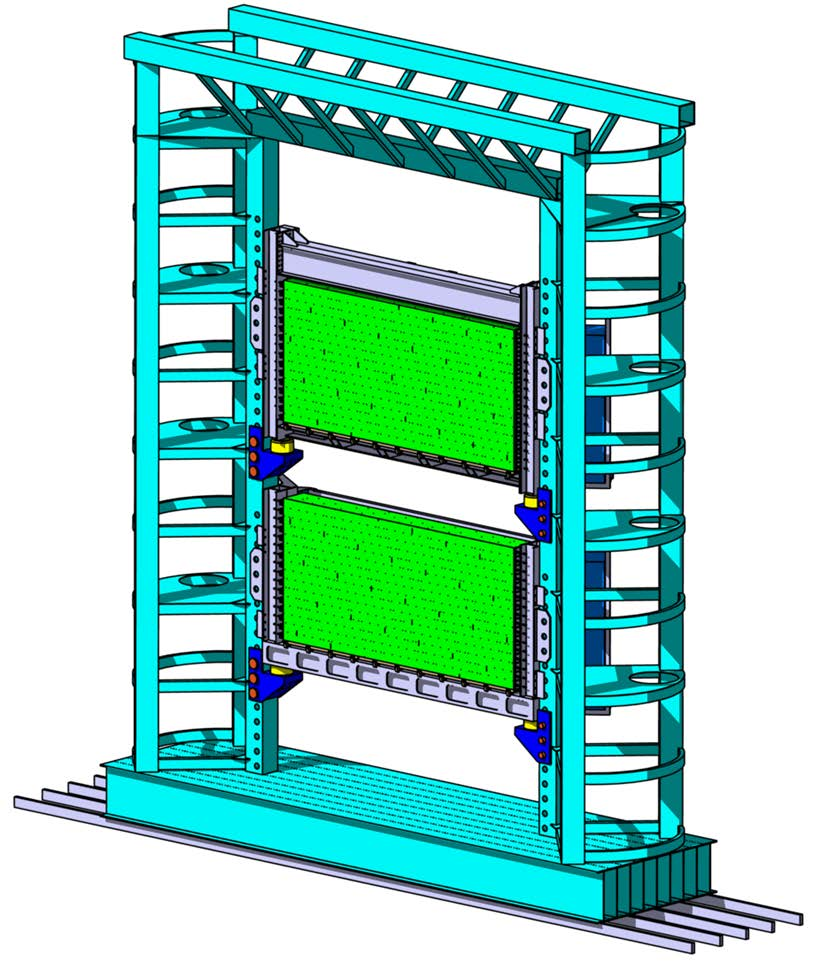
\includegraphics[width=0.95\textwidth]{pictures/CBM_ECAL_new.png}
\caption{Модель электромагнитного калориметра ECAL.}
\label{fig:ECAL}
\end{figure}
\end{minipage}
\begin{minipage}[t]{0.495\textwidth}
В эксперименте CBM будет установлен электромагнитный калориметр (Electromagnetic CALorimeter, ECAL) типа ``шашлык'', схожий с калориметрами экспериментов HERA-B, PHENIX и LHCb. Он будет использоваться для измерения прямых фотонов и нейтральных мезонов ($ \pi^{0}, \eta $), распадающихся на фотоны.
%Полный калориметр на SIS-300
ECAL будет собран из четырёхканальых модулей с поперечным сечением 12~см$\times$12~см, состоящих из 140 последовательных слоёв свинового абсорбера и пластикового сцинтиллятора толщиной 1~мм. Свет от сцинтилляторов собирается спектросмещающими волокнами, проходящими сквозь пачку свинца и пластика, и регистрируется ФЭУ, расположенными позади модулей. \\
%\small{The CBM electromagnetic calorimeter (ECAL) uses the ``shashlik'' technology. It is built from individual modules that are made from lead absorber plates interspaced with scintillator tiles as active material. Wavelength-shifting (WLS) fibers penetrate the lead/scintillator stack through holes, and readout at the back of sampling structure by photomultipliers.} \\
Взаимодействуя с материалом калориметра, налетающий фотон образует электромагнитный ливень. Таким образом первичный фотон полностью оставляет энергию в калориметре, где она собирается и измеряется. \\
%\small{Interacting with the material of the calorimeter, a photon produces a particle shower, which consists of electrons, positrons and secondary photons. In such a way the energy of the initial photon is deposited in ECAL, where it is collected and measured.} \\
%Планируется три типоразмера модулей: 3~см$\times$3~см, 6~см$\times$6~см и 12~см$\times$12~см. Модули могут быть организованы \\
%\small{A ``shashlik'' type calorimeter as installed in the HERA-B, PHENIX and LHCb experiments will be used to measure direct photons and neutral mesons ($ \pi^{0}, \eta $) decaying into photons. The full ECAL at SIS-300 will be composed of modules which consist of 140 layers of 1 mm lead and 1 mm scintillator, with cell sizes of 3 cm$\times$3 cm, 6 cm$\times$6 cm and 12 cm$\times$12 cm. The shashlik modules can be arranged either as a wall or in a tower geometry with variable distance from the target. To simplify the detector layout and to fit in a very limited budget for ECAL at SIS100 stage we have reduced the number of ECAL sections considering only 4-cell modules.}
%Конфигурация для SIS-100 имеет 4352~канала считывания, составленные из 1088~модулей одного типа (6~см$\times$6~см).
Калориметр, оптимизированный под установку на SIS100, составлен из 1088~модулей и имеет 4352~канала считывания. Модули сгруппированы в два прямоугольных блока, которые могут двигаться в вертикальном направлении, изменяя таким образом угловой диапазон измеряемых частиц и, следовательно, оптимизируя условия эксперимента для измерения различных первичных ионов при различных энергиях. \\
%\small{Optimized for SIS100 calorimeter system has 4352 electronic channels, built from 1088 modules of only one type (with $60 \times 60$ $mm^2$ cells). Calorimeter modules are grouped in two rectangular blocks which could be moved up and down (changing the angular range of measured particles and optimizing the experimental conditions for different colliding ion systems and beam energies).}
\end{minipage}

% ==========================================================================================================================
%__/\\\\\\\\\\\\\_______/\\\\\\\\\\\____/\\\\\\\\\\\\____        
% _\/\\\/////////\\\___/\\\/////////\\\_\/\\\////////\\\__       
%  _\/\\\_______\/\\\__\//\\\______\///__\/\\\______\//\\\_      
%   _\/\\\\\\\\\\\\\/____\////\\\_________\/\\\_______\/\\\_     
%    _\/\\\/////////_________\////\\\______\/\\\_______\/\\\_    
%     _\/\\\_____________________\////\\\___\/\\\_______\/\\\_   
%      _\/\\\______________/\\\______\//\\\__\/\\\_______/\\\__  
%       _\/\\\_____________\///\\\\\\\\\\\/___\/\\\\\\\\\\\\/___ 
%        _\///________________\///////////_____\////////////_____
% ==========================================================================================================================

\subsection{Детектор непровзаимодействовавших осколков PSD}\label{sec:secPSD}

% \todo Найти более новую картинку. Лучше никакая, чем такая. Написать Олегу.

\begin{minipage}[t]{0.495\textwidth}
\begin{figure}[H]
\centering
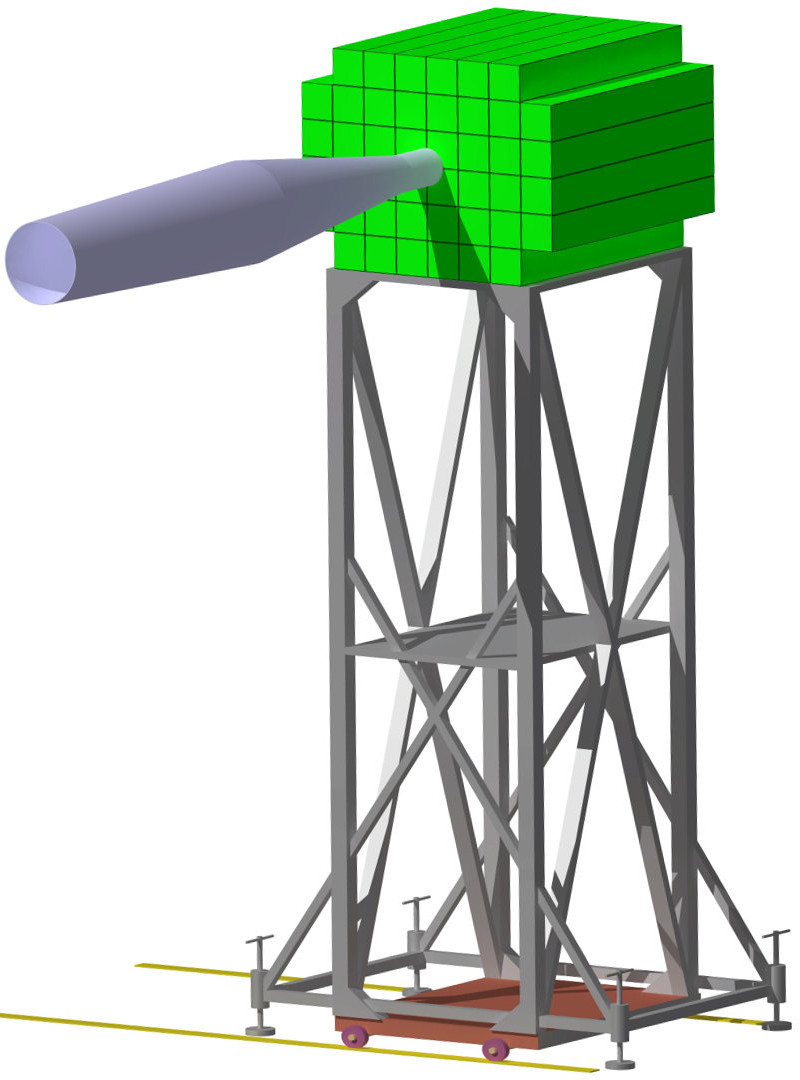
\includegraphics[width=0.95\textwidth]{pictures/CBM_PSD_model.png}
\caption{Модель калориметра PSD.}
\label{fig:PSD}
\end{figure}
\end{minipage}
\begin{minipage}[t]{0.495\textwidth}
Основная задача детектора непровзаимодействовавших осколков (Projectile Spectator Detector, PSD) --- выполнять измерения центральности столкновений тяжёлых ионов и ориентацию плоскости реакции. PSD представляет собой калориметр из свинца и сцинтиллятора, спроектированный для измерения распределения энергии налетающих осколков и летящих вперёд частиц. Основные технические требования к PSD --- покрытие углов от~$\SI{0.3}{\degree}$ до~$\SI{3}{\degree}$ и достаточное энергетическое разрешение для определения центральности столкновений, а также гранулярность в плоскости XY, необходимая для восстановления плоскости реакции. \\
%\small{The main purpose of the PSD is to provide an experimental measurement of a heavy-ion collision centrality and orientation of its symmetry plane. The PSD is a compensating lead-scintillator calorimeter designed to measure the energy distribution of the projectile nuclei fragments (spectators) and forward going particles produced close to the beam rapidity.
%The main design requirements of the PSD are
%(i) forward rapidity coverage and sufficient energy resolution to allow for precise collision centrality determination and consequently of the number of participating nucleons and
%(ii) granularity in the plane transverse to the beam direction which is needed for the collision symmetry plane reconstruction.}
% Выкинул слово compensating
\end{minipage}

В предлагаемом проекте детектор PSD составлен из 44~модулей и перекрывает такую поперечную площадь, чтобы большая часть непровзаимодействовавших фрагментов оставили всю свою энергию в детекторе. За счёт вытянутой в горизонтальном направлении геометрии детектор PSD позволяет регистрировать фрагменты, отклонённые магнитным полем дипольного магнита.

PSD предоставляет независимый метод для определения центральности соударения и множественности спектаторов.
PSD имеет разрешение по прицельному параметру, сравнимое с разрешением, предоставляемым кремниевой трековой системой STS и помогает улучшить определение центральности.

Разрешение по определению плоскости реакции с помощью PSD варьируется в диапазоне от $\SI{30}{\degree}$ до $\SI{40}{\degree}$ в зависимости от расстояния от мишени и энергии столкновения. С учётом предлагаемой вытянутой геометрии детектора и после коррекции нелинейности детектора в азимутальном направлении, разрешение практически не меняется в зависимости от силы поля дипольного магнита CBM.

%\small{The proposed 44 module design of the PSD covers large transverse area around the beam spot position such that most of the projectile spectator fragments deposit their energy in the PSD. The elongated transverse geometry of the PSD in horizontal direction takes into account the deflection of the fragments by the magnetic field of the CBM Dipole magnet. A lead-scintillator prototype of the PSD module with scintillator light readout by micropixel avalanche photodiodes and the PSD front-end electronics were tested with the proton and pion beams and cosmic muon rays. Radiation hardness and possible degradation of the PSD were studied with the FLUKA simulation of the CBM detector geometry.}

%\small{Depending on the collision energy, the PSD has a comparable impact parameter resolution to that of the CBM silicon tracking system (STS). Thus, the PSD provides an independent method in the CBM experiment of the centrality determination with spectator multiplicity. When used in a combination with the STS, the PSD helps to improve the overall centrality determination in the centrality range of 0--40\% and allows for centrality determination in narrow centrality classes with a width of at least 5\%.}

%\small{The PSD event plane resolution varies in the range of 30--40 degrees depending on the distance from the target and the collision energy. With the proposed elongated geometry, and after correction for the detector azimuthal non-uniformity, the resolution of the PSD event plane shows negligible variation with the field strength of the CBM magnet. We compared the PSD event plane resolution with that of STS and an alternative detector setup at forward rapidity such as a forward time of flight (TOF) detector. We concluded that the PSD has significantly better event plane resolution than both STS and forward TOF detector configurations.}
